% Clase del documento
\documentclass[12pt,twoside,titlepage]{report}





%%%%%%%%%%%%%%%%%%%%%%% Paquetes %%%%%%%%%%%%%%%%%%%%%%%

\usepackage[a4paper,bindingoffset=3mm,bottom=35mm]{geometry}


% Usad \usepackage[dvips]{graphicx} o \usepackage[pdftex]{graphicx} (no ambos)
%\usepackage[dvips]{graphicx} %%% para LaTeX. Las figuras deben estar en formato eps

\usepackage[colorlinks=true,pdftex]{hyperref}   %%% Opcional. Para incluir marcadores y enlaces en el pdf
\usepackage[pdftex]{graphicx}  %%% para pdflatex. Las figuras pueden estar en pdf, jpg, svg y otros formatos


\usepackage[spanish]{babel}

%\usepackage[latin1]{inputenc} % Usad en WinEdt/MikTex
\usepackage[utf8]{inputenc} % Usad en overleaf

%\usepackage[T1]{fontenc}


% Algunos paquetes útiles

\usepackage{amsmath,amssymb}
\usepackage{hyperref}
\usepackage{xcolor}
\usepackage{afterpage}
\usepackage{paralist}
\usepackage{array}
\usepackage{enumerate}
\usepackage{paralist}
\usepackage{enumitem}
\usepackage{float}
\usepackage{setspace}
\usepackage{listings}
\usepackage{algorithm}
\usepackage{algorithmic}
\usepackage{fancyhdr}
\usepackage{rotating}
\usepackage{multirow}


% Otros paquetes

\usepackage{quotchap}
\usepackage{lipsum}

%%%%%%%%%%%%%%%%%%%%%%%%%%%%%%%%%%%%%%%%%%%%%%%%%%%%%%%%






%%%%%%%%%%%%%%%%%%%%%%% Definiciones básicas %%%%%%%%%%%%%%%%%%%%%%%

\newcommand{\nombreautor}{Javier Raúl Alonso Tejera}
\newcommand{\nombretutor}{Michel Maes Bermejo}
\newcommand{\titulotrabajo}{OUTSIDER: UN JUEGO ONLINE EN TIEMPO REAL}
\newcommand{\escuela}{Escuela Técnica Superior\\de Ingeniería Informática}
\newcommand{\escuelalargo}{Escuela Técnica Superior de Ingeniería Informática}
\newcommand{\universidad}{Universidad Rey Juan Carlos}
\newcommand{\fecha}{Fecha}
\newcommand{\grado}{Grado en Ingeniería de Computadores}
\newcommand{\curso}{Curso 2023-2024}
\newcommand{\logoUniversidad}{logoURJC.pdf} % logoURJC.eps

%%%%%%%%%%%%%%%%%%%%%%%%%%%%%%%%%%%%%%%%%%%%%%%%%%%%%%%%%%%%%%%%%%%%






%%%%%%%%%%%%%%%%%%%%%%%%% Otras definiciones %%%%%%%%%%%%%%%%%%%%%%%%%%

% Definiciones de colores (para hidelinks)
\definecolor{BlueLink}{rgb}{0.165,0.322,0.745}
\definecolor{PinkLink}{rgb}{0.8,0.22,0.5}
\definecolor{gray}{rgb}{0.6,0.6,0.6}


% Enlaces
\hypersetup{hidelinks,pageanchor=true,colorlinks,citecolor=PinkLink,urlcolor=black,linkcolor=BlueLink}


\newcommand\blankpage{%
    \newpage
    \null
    \thispagestyle{empty}%
    %\addtocounter{page}{-1}%
    \newpage}


% Texto referencias
\addto{\captionsspanish}{\renewcommand{\bibname}{Bibliografía}}

% Texto Índice de tablas
\addto\captionsspanish{
\def\tablename{Tabla}
\def\listtablename{\'{I}ndice de tablas}
}


\floatname{algorithm}{Algoritmo}

\newfloat{algorithm}{t}{lop}

%% Etiquetas de comentarios (tutor/alumno)
\newif\ifdraft
\drafttrue
\usepackage{subcaption}
\newcommand{\nb}[2]{
	{
		{\color{black}{
				\small\fbox{\bfseries\sffamily\scriptsize#1}
				{\sffamily\small$\triangleright~${\it\sffamily\small #2}$~\triangleleft$}
	}}}
}

\ifdraft
\newcommand\tutor[1]{\nb{Tutor}{\color{red}#1}}
\newcommand\alumno[1]{\nb{Alumno}{\color{blue}#1}}
\newcommand\cotutor[1]{\nb{Co-tutor}{\color{green}#1}}
\newcommand{\fixme}[1]{{\textcolor{red}{[FIXME] #1}}\xspace}
\newcommand{\cn}{{\color{violet}[citation required]}}

\else
%\usepackage[disable]{todonotes}
\newcommand\tutor[1]{}
\newcommand\alumno[1]{}
\newcommand\cotutor[1]{}
\newcommand{\fixme}[1]{}
\newcommand{\cn}{}

\fi






%\newenvironment{pseudocodigo}[1][htb]
%  {\renewcommand{\algorithmcfname}{Pseudocódig}% Update algorithm name
%   \begin{algorithm}[#1]%
%  }{\end{algorithm}}
  
%%%%%%%%%%%%%%%%%%%%%%%%%%%%%%%%%%%%%%%%%%%%%%%%%%%%%%%%%%%%%%%%%%%%





%%%%%%%%%%%%%%%%%%%%%%% Estilo de código (en Python) %%%%%%%%%%%%%%%%%%%%%%%

\definecolor{bg}{rgb}{0.95,0.95,0.95}
\definecolor{mydeepteal}{rgb}{0.16,0.22,0.23}
\definecolor{myteal}{rgb}{0.31,0.44,0.46}
\definecolor{mymediumteal}{rgb}{0.41,0.58,0.60}

\DeclareFixedFont{\ttb}{T1}{txtt}{bx}{n}{12} % for bold
\DeclareFixedFont{\ttm}{T1}{txtt}{m}{n}{12}  % for normal


%\newcommand*{\FormatDigit}[1]{\textcolor{mydeepteal}{#1}}
\newcommand*{\FormatDigit}[1]{\textcolor{black}{#1}}

% Python style for highlighting
\newcommand\mypythonstyle{\lstset{
language=Python,
basicstyle=\ttfamily\small,
%basicstyle=\linespread{1.0}\footnotesize\ttm,
otherkeywords={self},             % Add keywords here
keywordstyle=\bfseries\ttfamily\color{myteal},
%keywordstyle=\ttb\color{myteal},
commentstyle=\itshape\color{myteal},
stringstyle=\color{mydeepteal},
emph={MyClass,__init__},          % Custom highlighting
emphstyle=\ttb\color{mydeepteal},    % Custom highlighting style
% Any extra options here
showstringspaces=false,            %
backgroundcolor=\color{bg},
rulecolor = \color{bg},
%identifierstyle=\color{deepgreen},
breaklines=true,
numbers=left,
numbersep=5pt,
numberstyle=\tiny,
tabsize=4,
xleftmargin=1em,
frame = single,
framesep = 3pt,
framextopmargin=0pt,
framexbottommargin=0pt,
framexleftmargin=0pt,
framexrightmargin=0pt,
fontadjust=true,
basewidth=0.55em, % compactness of code
upquote=true,
}}

% Python environment
\lstnewenvironment{mypython}[1][]
{
\mypythonstyle
\lstset{#1}
}
{}

\newcommand\mypythonstylenormalinline{\lstset{
language=Python,
basicstyle=\ttfamily\normalsize,
%basicstyle=\linespread{1.0}\footnotesize\ttm,
otherkeywords={self},            % Add keywords here
keywordstyle=\bfseries\ttfamily\color{myteal},
%keywordstyle=\ttb\color{myteal},
commentstyle=\itshape\color{mymediumteal},
stringstyle=\color{mydeepteal},
emph={MyClass,__init__},          % Custom highlighting
emphstyle=\ttb\color{mydeepteal},    % Custom highlighting style
% Any extra options here
showstringspaces=false,            %
backgroundcolor=\color{bg},
rulecolor = \color{bg},
%identifierstyle=\color{deepgreen},
breaklines=false,
numbers=left,
numbersep=5pt,
numberstyle=\tiny,
tabsize=4,
xleftmargin=0em,
frame = single,
framesep = 3pt,
framextopmargin=0pt,
framexbottommargin=0pt,
framexleftmargin=0pt,
framexrightmargin=0pt,
fontadjust=true,
%basewidth=0.55em, % compactness of code
upquote=true,
}}

\newcommand\mypythoninline[1]{{\mypythonstylenormalinline\lstinline!#1!}}

%%%%%%%%%%%%%%%%%%%%%%%%%%%%%%%%%%%%%%%%%%%%%%%%%%%%%%%%%%%%%%%%%%%%%%%%%%%%%%




%%%%%%%%%%%%%%%%%%%%%%%%%%%% Comandos definidos por el autor 

\newcommand{\transpuesta}{\mbox{\tiny $\mathsf{T}$}}








%%%%%%%%%%%%%%%%%%%%%%%%%%%%%%%%%%%%%%%%%%%%%%%%%%%%%%%%%%%%%%%%%%%%%%%
%                           Inicio del documento                       
%%%%%%%%%%%%%%%%%%%%%%%%%%%%%%%%%%%%%%%%%%%%%%%%%%%%%%%%%%%%%%%%%%%%%%%


\begin{document}

\pagestyle{plain}




%%%%%%%%%%%%%%%%%%%%%%%%%%%%%%%%%%%% Portada %%%%%%%%%%%%%%%%%%%%%%%%%%%%%%%%%%

%\pagenumbering{gobble}
%\pagenumbering{arabic}

% Universidad, Facultad
\begin{titlepage}
	\selectlanguage{spanish}
						
						
	% logo
	\begin{center}
		\includegraphics[scale=0.7]{\logoUniversidad}
	\end{center}
						
	\bigskip
						
	\begin{center}
		\begin{LARGE}
			\escuela \\
		\end{LARGE}
	\end{center}
						
	\bigskip
	\bigskip
						
	% Grado
	\begin{center}
		\begin{large}
			\textbf{\grado}\\
		\end{large}
	\end{center}
						
	% Curso
	\begin{center}
		\begin{large}
			\textbf{\curso}\\
		\end{large}
	\end{center}
						
	\bigskip
						
	\textbf{\begin{center}
		\begin{large}
			\textbf{Trabajo Fin de Grado}
		\end{large}
		\end{center}}
						
	\bigskip
	\bigskip
	\bigskip
						
	% Nombre del TFG
	\begin{center}
		\textbf{\begin{large}
			\MakeUppercase{\titulotrabajo}\\
			\end{large}}
	\end{center}
						
	% Nombre del autor
	\vspace{\fill}
	\begin{center}
		\textbf{Autor: \nombreautor}\\ \smallskip
		% Tutor
		\textbf{Tutor: \nombretutor}\\
		% Añadir segundo tutor si hubiera
												
												
		\bigskip
												
		% Fecha
		%\textbf{\fecha}\\
	\end{center}
\end{titlepage}


%%%%%%%%%%%%%%%%%%%%%%%% Opcional %%%%%%%%%%%%%%%%%%%%%%
%\blankpage

%\thispagestyle{empty}
%\begin{center}

% Nombre del trabajo
%\textbf{\begin{large}
%\MakeUppercase{\titulotrabajo}\\*
%\end{large}}
%\vspace*{0.2cm}
%\vspace{5cm}

% Nombre del autor y del tutor
%\large Autor: \nombreautor \\* \medskip
%\large Tutor: \nombretutor \\*

%\vfill

% Escuela, universidad y fecha
%\escuelalargo \\ \smallskip
%\universidad \\
%\vspace{1cm}
%\fecha \\

%\clearpage

%\end{center}
%%%%%%%%%%%%%%%%%%%%%%%%%%%%%%%%%%%%%%%%%%%%%%%%%%%%%%%%

\hypersetup{pageanchor=true}

\normalsize
\afterpage{\blankpage} % Se deben añadir página en blanco para que lo capítulos de la memoria o estas secciones introductorias empiecen en páginas impares

%%%%%%%%%%%%%%%%%%%%%%%%%%%%%%%%%%%%%%%%%%%%%%%%%%%%%%%%%%%%%%%%%%%%%%%%%%%%%%%





% Estilo de párrafo de los capítulos
\setlength{\parskip}{0.75em}
\renewcommand{\baselinestretch}{1.25}
% Interlineado simple
\spacing{1}

\pagenumbering{Roman}
\setcounter{page}{2}


%%%%%%%%%%%%%%%%%%%%%%%%% Agradecimientos o dedicatoria %%%%%%%%%%%%%%%%%%%%%%%%%%%

\chapter*{Agradecimientos}

Breves agradecimientos o dedicatoria.

\afterpage{\blankpage}

%%%%%%%%%%%%%%%%%%%%%%%%%%%%%%%%%%%%%%%%%%%%%%%%%%%%%%%%%%%%%%%%%%%%%%%%%%%%%%%%%%%






%%%%%%%%%%%%%%%%%%%%%%%%%%%%%%%%%%%% Resumen %%%%%%%%%%%%%%%%%%%%%%%%%%%%%%%%%%%%%%

\chapter*{Resumen}

Breve resumen del Trabajo de Fin de Grado (TFG). Recomendable entre 250-300 palabras, conteniendo los principales objetivos y resultados derivados del mismo.

\mbox{} \bigskip

\noindent \textbf{Palabras clave}:
\begin{compactitem}
	\item Python
	\item Ciberseguridad
	\item Aprendizaje automático (pueden ser varias)
	\item $\ldots$
\end{compactitem}

\afterpage{\blankpage}

%%%%%%%%%%%%%%%%%%%%%%%%%%%%%%%%%%%%%%%%%%%%%%%%%%%%%%%%%%%%%%%%%%%%%%%%%%%%%%%%%%%





%%%%%%%%%%%%%%%%%%%%%%%%%%%%%%%%%%%% Índices %%%%%%%%%%%%%%%%%%%%%%%%%%%%%%%%%%%%

% Estilo de párrafo de los Índices
\setlength{\parskip}{1pt}
\renewcommand{\baselinestretch}{1}
\renewcommand{\contentsname}{Índice de contenidos}


% Índice de contenidos
\tableofcontents
\afterpage{\blankpage}

% Índice de tablas (OPCIONAL)
% \listoftables
%  \afterpage{\blankpage}
% \addcontentsline{toc}{chapter}{\noindent \listtablename}

% Índice de figuras (OPCIONAL)
\listoffigures
\afterpage{\blankpage}
\addcontentsline{toc}{chapter}{\listfigurename}

% Índice de códigos/algoritmos (OPCIONAL).   El término "Códigos" se puede cambiar por "Métodos", "Funciones", "Algoritmos", etc.
\renewcommand\lstlistlistingname{Códigos}
\renewcommand\lstlistingname{Código}
\renewcommand\lstlistlistingname{Índice de códigos}

\lstlistoflistings
\afterpage{\blankpage}
\addcontentsline{toc}{chapter}{\lstlistlistingname}


% En este documento (de momento) no se ha considerado incluir un índice de algoritmos/pseudocódigos, como el que aparece en \ref{AdditionalLouvain}

%%%%%%%%%%%%%%%%%%%%%%%%%%%%%%%%%%%%%%%%%%%%%%%%%%%%%%%%%%%%%%%%%%%%%%%%%%%%%%%%%%%





%%%%%%%%%%%%%%%%%%%%%%% Cabeceras y pies de página (Opcional) %%%%%%%%%%%%%%%%%%%%%%%

%\setlength{\headheight}{15.2pt}
\pagestyle{fancy}


\renewcommand{\chaptermark}[1]{\markboth{Capítulo \thechapter.\ #1}{}}

\pagestyle{fancy}
\fancyhf{}
\fancyhead[LO]{\leftmark}
\fancyhead[RO]{}
\fancyhead[RE]{\nouppercase\rightmark}
\fancyhead[LE]{}
\fancyfoot[C]{\thepage}

%%%%%%%%%%%%%%%%%%%%%%%%%%%%%%%%%%%%%%%%%%%%%%%%%%%%%%%%%%%%%%%%%%%%%%%%%%%%%%%%%%%%






%%%%%%%%%%%%%%%%%%%%%%%%%%%%%% Capítulos de la memoria %%%%%%%%%%%%%%%%%%%%%%%%%%%%%



% Capítulo 1
\chapter{Introducción}


%%%%%%%%%%%%%%%%%%%%%%%%%%%%%%%%%%%%%%%%%%%%%%%%%%%%%%%%%%%%%%%%%%%%%%%%%%

% Estilo resto de páginas
\pagestyle{fancy}


% Estilo de párrafo de los capítulos
\setlength{\parskip}{0.75em}
\renewcommand{\baselinestretch}{1.25}
% Interlineado simple
\spacing{1}
% Numeración contenido
\pagenumbering{arabic}
\setcounter{page}{1}

%%%%%%%%%%%%%%%%%%%%%%%%%%%%%%%%%%%%%%%%%%%%%%%%%%%%%%%%%%%%%%%%%%%%%%%%%%

Este documento aborda y explica el desarrollo de este proyecto de fin de grado,
desde su concepción inicial y las motivaciones que lo impulsaron, hasta los detalles
finales de su implementación.

\section{Descripción general}

El objetivo general del proyecto es el desarrollo de un juego multijugador web de adivinanza de palabras y roles ocultos. El principal punto de interés
radica en el uso de tecnologías en tiempo real, específicamente de tecnologías websocket, posibilitando el juego online entre los jugadores
de forma fiable y óptima.

Las mecánicas base del juego son sencillas y son más una adaptación de un tipo de juego que normalmente se realiza sin el uso de tecnologías informáticas.
El concepto más básico del juego se podría resumir mediante los siguientes puntos:

\begin{enumerate}
	\item En este juego, todos los jugadores juegan como ``Inocentes'', a excepción de uno de ellos,
	      definido como el ``Outsider''.
	\item Al empezar la partida, los jugadores
	      Inocentes reciben una
	      palabra secreta o contraseña, como por ejemplo, ``Hoja''.
	\item  Siguiendo un orden secuencial (con el primer jugador elegido al azar), cada
	      participante debe escribir una palabra relacionada con su palabra clave
	      para indicar a los demás que conocen la palabra asignada.
	\item Por ejemplo si la palabra clave es la palabra ``Hoja'', unas palabras que
	      alienten a esta  o palabra clave podrían ser ``Árbol'', ``Libro'' o ``Afeitado''.
	\item El jugador designado como Outsider, quien no tiene conocimiento de la palabra secreta, debe tratar de deducirla a partir de las palabras
	      previamente mencionadas y decir una palabra que no levante sospechas.
	\item Después de que todos los jugadores hayan compartido una palabra, se lleva a cabo una votación simultánea, donde cada jugador vota por la persona que creen
	      que es el Outsider.
	\item El Outsider ganará si no es el jugador más votado. Por otra parte, el resto de los jugadores Inocentes ganarán
	      si logran descubrir al Outsider y este llega a ser el jugador más votado.
\end{enumerate}

Dadas estas reglas de funcionamiento del juego, el desarrollo del proyecto consiste principalmente en
interpretar y diseñar una aplicación web capaz de poder gestionar todos estos puntos. En el próximo capítulo de Objetivos (\ref{Objetivos}),
se tratará con más detalle esta definición de reglas.

Además de generar una aplicación/juego que emule estas reglas, es bastante destacable el trabajo adicional relacionado con la gestión informática que
implica desarrollar una aplicación web: desde el diseño de interfaces usables hasta su despliegue y testeo, todos estos apartados se trataran en detalle
como parte del desarrollo.

\section{Motivación}

La principal motivación para la realización de este proyecto es el aprendizaje propio. La idea del juego
surge por parte del tutor del TFG, \nombretutor, que ve muy interesante la creación de una aplicación que haga uso de tecnologías en
tiempo real. También ha sido una figura clave en el desarrollo iterativo del proyecto, proponiendo mejoras y comentarios
a las diferentes versiones de la aplicación.

Dicho esto, a día de hoy hay innumerables proyectos, aplicaciones y juegos que persiguen conseguir un rendimiento económico o lúdico, sin embargo, también es importante destacar el papel
de la investigación y el aprendizaje, especialmente en el ámbito académico en el que se sitúa este trabajo de fin grado.

Las empresas y organizaciones buscan desarrolladores software altamente capacitados, pero también especializados en materias en concreto.
Destaca más un desarrollador que sepa sobre una tecnología útil y difícil de aprender sobre otro que sepa
sobre otra tecnología menos útil o mucho más accesible. Aquí es donde entran en juego los websockets, cuyas implementaciones suelen dar problemas 
a los desarrolladores.

Muchos estudiantes hemos realizado pequeños proyectos y pruebas con websockets y tecnologías análogas, pero es muy diferente desarrollar toda una aplicación, realizar testing e
incluso llevar a cabo un despliegue en torno a tecnologías en tiempo real. Hay que tener en cuenta muchas variables y por otra parte se tratan de tecnologías útiles
con infinidad de aplicaciones. Desde un simple chat en línea al uso de websockets en grandes proyectos, el uso de aplicaciones web en tiempo real es muy práctico.

Desde mi experiencia previa en desarrollo de aplicaciones móviles, un desarrollador no es consciente de la cantidad de lógica que se necesita para manejar una base
de datos en lo que a priori se presenta como una sencilla aplicación. Todo el trabajo subyacente es muy poco conocido pero suele ser de gran importancia. En este trabajo previo,
se destaca que se planteó varias veces la necesidad de poder crear conexiones websockets entre usuarios de la aplicación para poder compartir datos de forma inmediata.

Las aplicaciones que usamos en nuestros teléfonos y dispositivos, los videojuegos online o los servicios de streaming 
dependen de una estructura muy bien pensada para cada caso específico. Por ello, es una necesidad por parte de un desarrollador software, 
al menos entender, como funcionan todos estos sistemas. Mi objetivo es explorar y aprender lo máximo de la mayor cantidad de tecnologías 
software para desarrollarme como profesional así como para enseñar las posibilidades que ofrecen estas diversas herramientas.


% \afterpage{\blankpage} % puede generar problema en índice de contenidos
% \newpage

% Capítulo 2
\chapter{Objetivos}
\label{chap:objetivos}
En esta sección se definirán los objetivos principales del proyecto así como de otros objetivos y
requisitos secundarios que han ido definiéndose a lo largo del proyecto.

\section{Objetivos funcionales del juego} \label{Objetivos}

En primera instancia destacamos las funcionalidades básicas que debería cumplir el juego como
producto software, es decir, relacionados con el usuario de forma directa.

\subsection{Funcionalidad básica, lobby y conexiones}

Además del propio juego, es necesario dar las capacidades y herramientas necesarias a los usuarios para
poder organizar partidas de forma sencilla. Para ello se plantea la creación de una página de inicio que
permita al usuario poder crear salas de juego o unirse a salas ya creadas.

El objetivo en detalle sería permitir a todos los usuarios de la aplicación poder jugar a
diferentes partidas, teniendo en cuenta varias limitaciones como el que un jugador no debería poder acceder
a una partida ya empezada o evitar la creación de salas con el mismo nombre. De forma adicional, en esta página se deberían mostrar instrucciones que expliquen el funcionamiento
del juego.

También sería esencial tener una pantalla pre-partida en la cual se vayan uniendo los jugadores
antes de comenzar el juego. En esta pantalla se propone añadir un chat para los jugadores además
de mostrar la información pertinente al estado de la partida: número de jugadores preparados, código de la
sala para que se puedan unir más jugadores, etc.

\subsection{Juego sencillo}

En primer lugar, se plantea poder jugar de forma sencilla solo una ronda en la cual se deciden los
roles de los jugadores y se les indica una palabra clave a los jugadores Inocentes. Esta palabra 
clave es desconocida por el Outsider y el resto de jugadores Inocentes deberán demostrar 
que la conocen mientras evitan desvelarla al verdadero jugador Outsider. Se destaca 
que ninguno de los jugadores debería conocer a ciencia cierta el rol de otro, por ello, se trata de un juego 
con un alto factor de interacción social, donde la intuición y la discreción son elementos clave.

Con la palabra clave revelada a los jugadores Inocentes, se procede con la lógica de juego estándar: cada jugador siguiendo 
un orden secuencial, escribirá una palabra relacionada con su palabra clave
para indicar a los demás que conocen la palabra asignada; después de que todos los jugadores hayan compartido una
palabra, se lleva a cabo una votación simultánea, donde cada jugador vota por la persona que creen
que es el Outsider.

El Outsider ganará si no es el jugador más votado. Por otra parte, el resto de los jugadores Inocentes ganarán
si logran descubrir al Outsider y este llega a ser el jugador más votado.

El objetivo es llevar a cabo la implementación de esta lógica de la forma más consistente posible, trabajando en
detalle las conexiones websocket.

\subsection{Última oportunidad}

Habiendo implementado el juego sencillo, se quiere añadir nuevas funcionalidades base. En primer lugar, dado el transcurso
normal del juego, tras la votación simultánea, en el caso de que el Outsider reciba la mayoría de los votos, se le otorgará
una última oportunidad para ganar adivinando la palabra clave.

\subsection{Múltiples rondas}

Cuando existen más de tres jugadores en una partida, se detecta la necesidad de poder jugar varias rondas,
ya que, si no se elimina al Outsider inicialmente y se elimina a un jugador Inocente, podrían seguir jugando el resto de jugadores
rondas adicionales.

Los jugadores eliminados pasan a ser espectadores mientras el resto sigue jugando hasta que no 
se pueda seguir el juego porque solo queden un jugador Outsider y otro Inocente (en este caso
ganaría el Outsider de forma definitiva) o se elimine mediante votación al Outsider en cuestión.

\subsection{Varios Outsider}

Relacionado con el anterior punto, en partidas con varios jugadores se ve necesario aumentar el número de Outsiders en aras de
una jugabilidad más interesante. De esta manera, se plantea que cuando el número de jugadores sea mayor que seis, simplemente sean
dos jugadores Outsider en la partida.

En estos casos el Outsider solo tendrá la oportunidad de adivinar la palabra clave si es el último Outsider en la partida. Por contraparte, si 
todavía hay dos Outsiders jugando y solo quedan otros dos jugadores Inocentes sin eliminar, ganaría el bando Outsider al tener ventaja en los 
votos.

\section{Objetivos secundarios y tecnológicos}

Dados los objetivos/reglas principales que debería cumplir el juego, se añaden varios puntos adicionales que se quieren
tratar como objetivos secundarios del proyecto.

\subsection{Plataforma de juego}

Se quiere aprovechar el uso de un entorno web para hacer más accesible el juego a diferente tipo de usuarios.

El objetivo es hacer usable la aplicación en el mayor número de dispositivos posibles diferenciando principalmente entre
teléfonos móviles y equipos de escritorio (ordenadores y portátiles esencialmente). Se diferencia entre estos dos tipos de
dispositivos porque también se prevén dos tipos de juego de forma predominante:

\begin{compactitem}
    \item Juego presencial en un mismo espacio físico.
    \item Juego remoto.
\end{compactitem}

Se entiende que si un grupo quiere jugar en un espacio físico común, por ejemplo, en un cumpleaños en la casa de uno de los
jugadores, en la mayoría de casos todos los jugadores jugarán con sus propios dispositivos móviles, principalmente smartphones.

Por otro lado, también se ve bastante común que otro grupo de jugadores quiera jugar de forma remota, cada uno en una
localización diferente. En este caso, se podría asumir que la mayoría de jugadores intentarían jugar con sus dispositivos de
escritorio.

\subsection{Testing}

Se propone de forma adicional trabajar ciertos elementos de Integración Continua (CI, por sus siglas en inglés), especialmente el testing del software, ya que, es una práctica
esencial en la industria y resulta bastante llamativo trabajar el testing con tecnologías en tiempo real.

\subsection{Despliegue}

Para poder enseñar el resultado del proyecto de la forma más accesible posible, también se quiere trabajar con tecnologías de
AWS (Amazon Web Services) para poder tener la aplicación desplegada y totalmente disponible para cualquier usuario a la hora
de acceder a esta.

De esta forma se pretende aprender sobre tecnologías de despliegue y de crear una mejor presentación final del proyecto.

\subsection{Feedback de usuarios}

Para finalizar con la descripción inicial de objetivos, se pretende realizar una pequeña prueba con usuarios a mitad de
desarrollo con el objetivo de encontrar bugs y pequeñas mejoras para el juego, lo que generará su propia lista de cambios a realizar.

\section{Resumen de objetivos}

\begin{enumerate}
    \item Gestionar las conexiones entre jugadores mediante salas.
    \item Creación del juego básico.
    \item Añadir una mecánica adicional a la hora de eliminar al último jugador Outsider.
    \item Permitir jugar varias rondas.
    \item Añadir más jugadores Outsider al juego si hay muchos jugadores en partida.
    \item Gestionar la usabilidad de la aplicación en diferentes dispositivos.
    \item Tener en cuenta el feedback de los usuarios. Testing manual.
    \item Realización de tests para la lógica en tiempo real. Testing automático.
    \item Desplegar la aplicación a través de tecnologías modernas.
\end{enumerate}

\blankpage

% Capítulo 3
\chapter{Herramientas y Metodología}
\label{chap:herramientas}
A continuación se expondrá brevemente el uso de tecnologías así como la metodología
de trabajo que se ha seguido para la elaboración de la aplicación.

\section{Herramientas y tecnologías usadas}

\subsection{Django - Django Channels}

Las bases del proyecto se fundamentan en el uso de Django \cite{django} como tecnología de backend.

Además de conocer en profundidad cómo funcionan este framework y Python (que es el lenguaje con el que trabaja Django),
esta se trata de una herramienta que permite un desarrollo rápido, seguro y escalable.

Por otra parte se trabajará con Django Channels \cite{djangoChannels} para gestionar el uso de websockets. Django Channels
permite el uso de websockets y tecnologías análogas mediante varios paquetes \alumno{en la documentación se hace uso
directo del término paquete o módulo 'Channels is comprised of several packages...' son prácticamente sinónimos pero como veas} que se integran dentro del framework de Django.
A través del uso de 'consumers' o consumidores, abstracciones propias de Channels, 
se desarrollará la mayor parte de la lógica de la aplicación. 

Posteriormente se hará mención a Pytest \cite{pytest} a la hora de implementar el testing automático.

\subsection{Vue3}

Por otro lado, para el desarrollo frontend se propone el uso de Vue \cite{vue3} debido a su popularidad, versatilidad
y a su uso personal en otros proyectos. De esta forma se creará un frontend sencillo pero bastante personalizable.

Se hace referencia a Vue3 por ser la versión más moderna de Vue, la cual tiene cambios destacables en comparación
a Vue2 \cite{vue3vue2}. Todos los paquetes y librerías adicionales se incorporarán teniendo en cuenta que se está haciendo uso de
Vue3. En especial, se destaca la librería de componentes Vuetify \cite{vuetify}, la cual es un gran añadido a la hora de
ofrecer una gran diversidad de componentes para la construcción de una interfaz vistosa y dinámica.

\subsection{Herramientas de diseño}

Figma \cite{figma} es un editor de gráficos que se usa principalmente para generar prototipos. Se usará principalmente para
el diseño y experimentación inicial de la aplicación web. Además de Figma, se harán uso de otras herramientas
menores de diseño como draw.io \cite{draw.io} para la creación de diagramas, Pictogrammers \cite{pictogrammers} para hacer uso de
iconos de forma sencilla o Contrast Finder \cite{contrastFinder} para comparar contrastes de color.

\subsection{Docker}

Docker \cite{docker} es una herramienta de código abierto que facilita un despliegue sencillo y portable utilizando contenedores
virtuales. Estos contenedores se emplearán para hospedar los diversos servicios del sistema en un
servidor.

\subsection{AWS}

Amazon Web Services (AWS)~\cite{aws} es una plataforma de servicios en la nube ofrecida por Amazon. Proporciona
una amplísima gama de servicios que incluyen computación, almacenamiento, bases de datos, ... Estas soluciones permitirán
alojar la aplicación final de forma flexible y sencilla.

Se detallará el uso tanto de Docker como de AWS en el proceso de preparación y despliegue de la aplicación.

\subsection{GitHub}

GitHub \cite{github} es una plataforma de desarrollo colaborativo basada en la web que utiliza Git, un sistema de control de versiones
distribuido. Permite a los desarrolladores alojar, gestionar y compartir proyectos de software, facilitando la accesibilidad
del código.

Todo el código del proyecto será accesible mediante un repositorio público en GitHub \cite{repositorio} .

\subsection{WSL}

Se destaca de forma adicional el uso del subsistema de Windows para Linux (WSL) \cite{wsl} para poder ejecutar de forma sencilla
todo el entorno de la aplicación así como para la realización de pruebas de despliegue sin dejar de hacer uso directo de Windows
como sistema operativo.

\subsection{Visual Code}

En último lugar se encuentra la herramienta más básica y a la vez más importante para
el proyecto, Visual Studio Code \cite{vscode}. Visual Studio Code, comúnmente conocido como Visual Code o VS Code,
es un editor de código fuente desarrollado por Microsoft.

Todo el código se ha tratado mediante Visual code, desde la creación y edición del código hasta la ejecución de comandos
de terminal.


\section{Metodología}

Este proyecto se ha guiado por el uso de una metodología de trabajo iterativa-incremental enfocada en la revisión de objetivos y
avances entre el tutor y el alumno. Durante cada encuentro, se han ido discutiendo propuestas de mejora que se han convertido en
objetivos para la siguiente evaluación. En primera instancia se han planteado unos objetivos principales (crear el juego
con funcionalidades básicas) y diversos objetivos adicionales/opcionales que se han ido discutiendo e
implementando a lo largo de las diferente reuniones (testing, mecánicas adicionales, despliegue mediante AWS, ...).

Esta metodología ha demostrado ser efectiva para este tipo de proyecto, ya que permite un avance progresivo y detallado,
evitando la acumulación de muchas tareas. Además, al planificar con visión a futuro, la aplicación ha crecido de manera sólida
y constante, sin necesidad de realizar cambios radicales.


% Capítulo 4
\chapter{Descripción informática}
\label{chap:descripInfor}
En esta sección se expondrá la mayor cantidad de información sobre el desarrollo per se
del proyecto, desde la definición de requisitos y análisis inicial, hasta el proceso final
de testing y despliegue.

\section{Requisitos}

Definidos los objetivos del proyecto y tras realizar una primera reunión
con el tutor del TFG, \nombretutor, se pueden definir de forma más concisa tanto los
requisitos funcionales como los no funcionales que debe cumplir la aplicación.

\subsection{Requisitos funcionales}

Una posible estructura de la memoria final asociada con cada TFG podría ser la siguiente (leed la normativa de TFG):
\begin{itemize}
	\item RF1 Página de inicio - Debe existir una página principal que permita establecer el nombre dentro del juego al usuario,
	      que explique las reglas de juego y que establezca una interfaz sencilla para poder crear o unirse a una sala.
	\item RF2 Creación de salas - Un usuario debe ser capaz de crear una sala y también poder unirse a salas ya creadas mediante un
	      código único.
	\item RF3 Sala de juego y chat - Dentro de una sala, cada jugador debe poder visualizar a todos los jugadores con los que va a jugar
	      así como interactuar con ellos de forma sencilla mediante un chat.
	\item RF4 Empezar partida - Dado un número mínimo-máximo de jugadores uno de los jugadores debería tener la capacidad
	      para empezar una nueva partida.
	\item RF5 Conexiones - Tiene que existir una lógica que asuma conexiones o desconexiones accidentales y deliberadas por parte
	      de alguno o varios jugadores antes de empezar la partida en la sala, durante el juego o en la visualización de resultados.
	\item RF6 Inicio de partida - Al empezar la partida, el sistema debería proporcionar un orden aleatorio de turnos secuencial además de
	      la asignación de un rol junto a la contraseña a los jugadores Inocentes.
	\item RF7 Turnos - El orden secuencial a la hora de enviar palabras debería ser visible y destacar cuando es el turno
	      de un jugador en concreto.
	\item RF8 Enviar palabras - De forma secuencial, todos los jugadores deberían poder enviar una palabra semejante a la pista asumiendo
	      el juego de roles Outsider/Inocente sin interferencias por parte de otros jugadores.
	\item RF9 Votaciones - Al finalizar el envio de palabras se asume una fase de votaciones en la que, de forma asíncrona,
	      cada jugador vota a otro con el fin de acusarlo de Outsider y eliminarlo del juego.
	\item RF10 Resultados - Habiendo votado todos los usuarios, el sistema calcularía el resultado de esta votación para definir el
	      desenlace final de la ronda y se les mostraría a cada uno de los jugadores de forma simultánea este resultado.
	\item RF11 Gameloop - El sistema debe identificar cuando todos los jugadores han enviado sus palabras, mostrar la interfaz
	      de votación y finalmente gestionar y revelar los resultados a todos los jugadores de forma consistente.
	\item RF12 Varias rondas - Si el número de jugadores  y el resultado de la ronda lo permite, el sistema debe asumir que tras
	      la finalización de una ronda pueden jugarse otras rondas de forma adicional si se desea. Por ejemplo, si hay cuatro jugadores y los tres jugadores
	      Inocentes no han identificado/votado al Outsider de forma correcta, se podría jugar otra ronda con tres jugadores si se ha votado de forma
	      errónea a un jugador Inocente o con los mismos cuatro si ha habido un empate en la votación.
	\item RF13 Varios Outsider - Si el número de jugadores es bastante alto, el sistema asignará el rol de Outsider a otro jugador de forma adicional.
	\item RF14 Última oportunidad - En el caso en el que el jugador con más votos sea el último Outsider en la partida, este tendrá un intento de
	      adivinar la contraseña que conocen los jugadores Inocentes.
	\item RF15 Multiplataforma - La aplicación debe ser accesible desde diferntes tipos de dispositivos como telefónos móviles u ordenadores portátiles
	      y de sobremesa.
\end{itemize}

\subsection{Requisitos no funcionales}

\begin{itemize}
	\item RNF1 Usabilidad y accesibilidad básicas - La aplicación web debe atender a valores de usabilidad universales, como el uso del zoom o
	      el de diferentes resoluciones así como accesibilidad básica como el uso de colores con contraste por ejemplo.
	\item RNF2 Calidad de las conexiones - Se debe tener en cuenta la calidad y estabilidad de las conexiones mediante websocket para evitar
	      interrumpir, en la medida de lo posible, a los jugadores.
	\item RNF3 Información de estado - Se debe mantener informado al usuario del estado general de la partida así como de las posibles conexiones y desconexiones
	      por parte de otros jugadores.
	\item RNF4 Testing - El sistema tendrá una opción de desarrollo para poder ejecutar diversos tests que ponen
	      a prueba el correcto transcurso de una partida así como las conexiones y desconexiones en el entorno websocket del backend.
	\item RNF5 Despliegue y administración - La aplicación estará lsita para el despliegue y accesible para poder tener información de administración del servidor
	      backend.
	\item RNF6 Documentación - Todas las capacidades de administración actuales y de futuro desarrollo serán accesible de forma sencilla.
\end{itemize}

\section{Arquitectura general}

En este apartado, se pretende definir de forma más concisa la arquitectura software de la aplicación
teniendo en cuenta las tecnologías usadas y su interoperabilidad además del por qué se han tomado estas decisiones de diseño.

Después de haber analizado los diferentes requisitos y considerando las herramientas y conocimientos de partida,
se definen los servicios mínimos que debería ofrecer el sistema en conjunto:

\begin{enumerate}
	\item Backend - Django. Para empezar, es fundamental el uso de un servidor backend capaz de
	      gestionar la lógica de peticiones básica y que tenga capacidad para hacer uso de tecnología websocket.
	      Para esta tarea, se propone una implementación sencilla a través de Django. Se destaca que hay muy poca información que se
	      quiera tratar de forma persistente, por ello, no será necesario un servicio de base de datos adicional
	      y se recurrirá a la configuración por defecto de Django con un archivo SQLite.
	\item Servidor websocket - Redis (Django Channels). Al hacer uso de Django y de su particular implementación de
	      websockets, se ve indispensable el uso de un servicio adicional, un servidor redis. Este servidor es necesario para
	      poder hacer uso del sistema de 'capas', que permiten que varias instancias de controladores websocket
	      (denominados 'consumers') puedan comunicarse entre sí y con otras partes de Django \cite{djangoChannelsLayers}.
	\item Frontend - Vue3. Finalmente, solo quedaría gestionar la vista de la aplicación a través de Vue
	      que, para el desarrolador, facilita mucho el trabajo de frontend, integrando una gran cantidad de herramientas y componentes.
	      Dentro de este servicio se tendrá que trabajar la comunicación con el backend así como la visualización y lógica
	      web, por ejemplo, la lógica de navegación entre páginas a través de vue-router.
\end{enumerate}

Estos serían los elementos básicos del sistema, pero hay que tener en cuenta su
despliegue final. Para entenderlo todo de forma más organizada en la figura \ref{fig:res_arquitecturaSoftware} se muestra un esquema de la arquitectura
a nivel general. En el apéndice se muestra la misma imagen (\ref{fig:res_arquitecturaSoftware}) de mayor tamaño.

\begin{figure}[h]
	\centering
	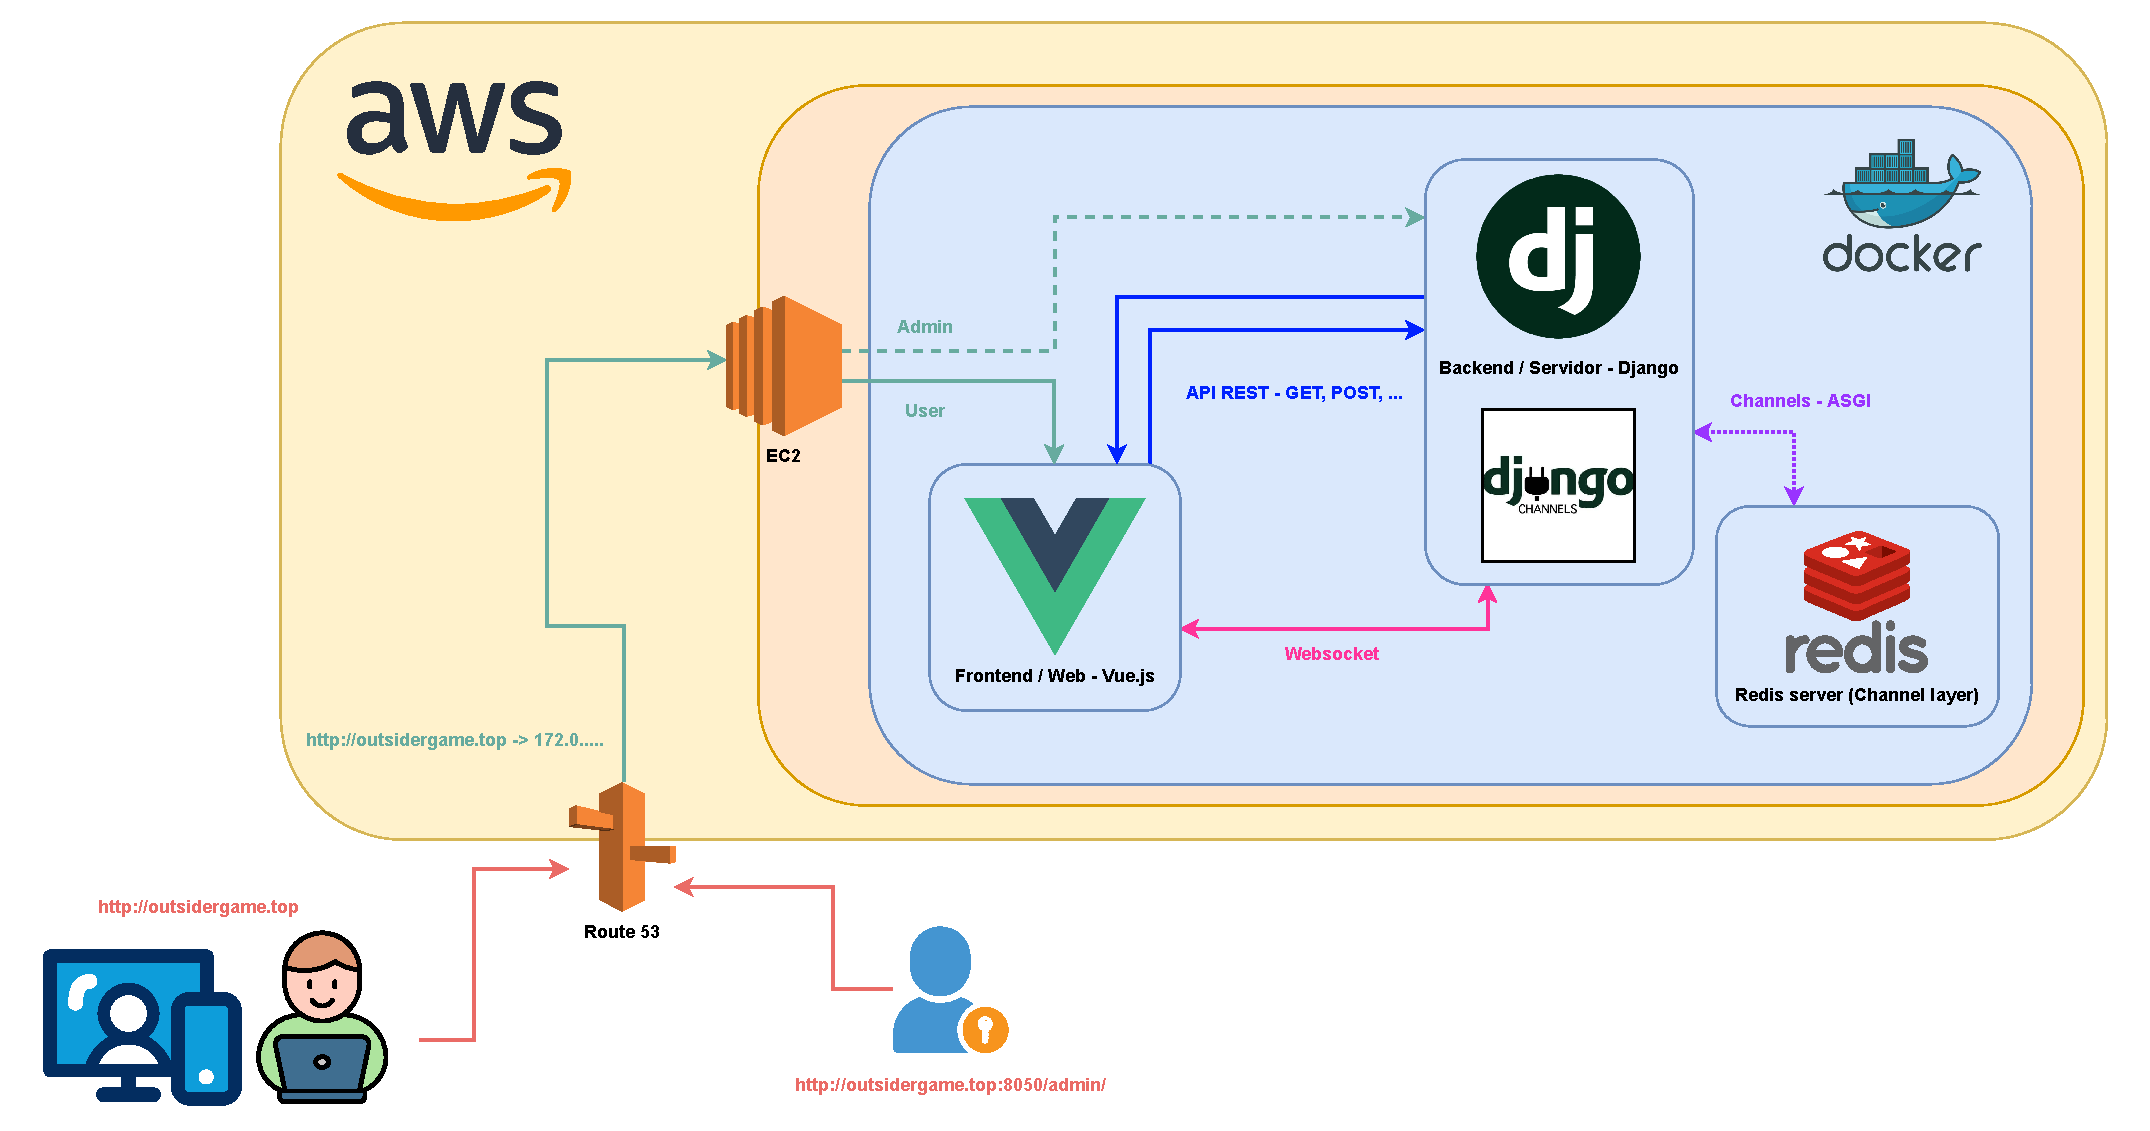
\includegraphics[width=\textwidth,clip=true]{res_arquitecturaSoftware.pdf}
	\caption{Arquitectura final del sistema}
	\label{fig:res_arquitecturaSoftware}
\end{figure}

De este esquema inicial cabría destacar un poco más en detalle el funcionamiento de las conexiones websocket, ya que, Django Channels 
está construido sobre la especificación ASGI (Asynchronous Server Gateway Interface), diseñada para proporcionar una interfaz estándar entre servidores web Python, frameworks y aplicaciones que soportan asincronía \cite{ASGI}. Dicho de otra forma,
permite hacer uso tanto de conexiones y peticiones HTTP como del uso del protocolo websocket sin problemas, algo totalmente nencesario para el desarrollo del proyecto. 

Dicho esto, la comunicación a bajo nivel se hace un poco más enrevesada, ya que, lo que facilita Django Channels son las herramientas de alto
nivel para trabajar directamente con los websockets. En la figura \ref{fig:res_esquemaDjangoChannels} se puede observar con mayor detalle como funcionan
las conexiones a bajo nivel en el entorno ASGI de Channels \cite{whatIsDjangoChannels}. De esta forma se puede entender un poco más sobre como funcionan las 
conexiones a bajo nivel respecto al anterior esquema general, el cual solo hace referencia a las conexiones de alto nivel entre los servicios principales de la aplicación.

\begin{figure}[h]
	\centering
	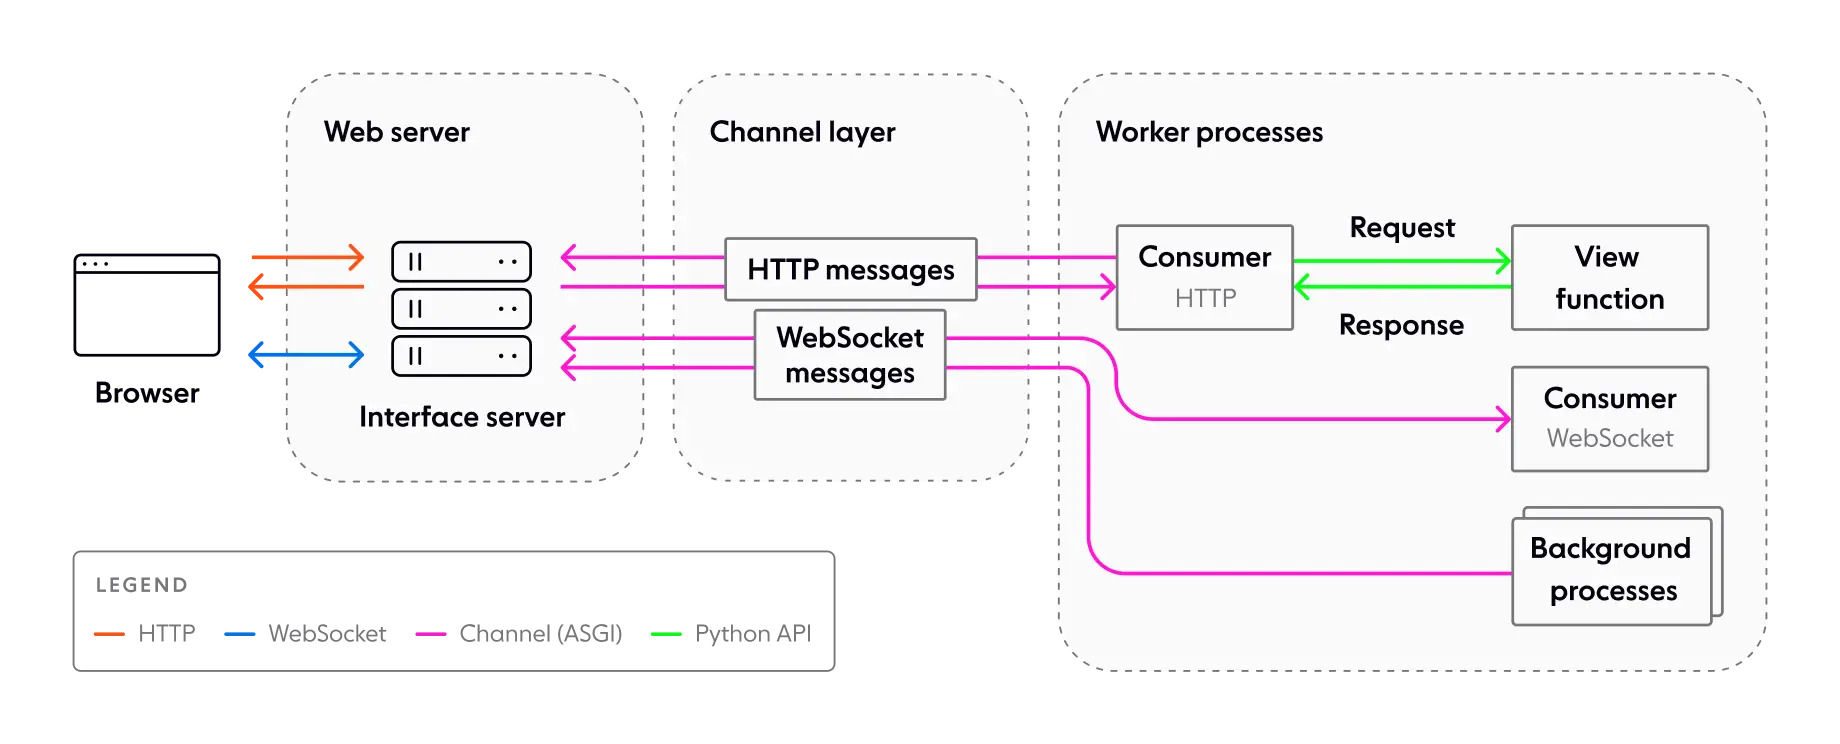
\includegraphics[width=\textwidth,clip=true]{res_esquemaDjangoChannels.jpg}
	\caption{Arquitectura de Django Channels}
	\label{fig:res_esquemaDjangoChannels}
\end{figure}

Obviando la comunicación ASGI a bajo nivel y los elementos asociados al despliegue (que se trataran con más detalle en las siguientes secciones), el resto del esquema es más sencillo: El usuario utilizará una URL, 
\href{http://outsidergame.top/}{outsidergame.top}  para acceder a la aplicación web y hacer uso de esta. La aplicación web (Vue) hará las necesarias comunicaciones (tanto HTTP como websocket) 
para acceder al contenido y la lógica del juego contenidas en el servidor de Django/Channels. De forma adicional se dispone una URL de administrador, 
\href{http://outsidergame.top:8050/admin/}{outsidergame.top:8050/admin/} protegida con credenciales para que el supuesto administrador de la web 
pueda gestionar algún dato de forma directa (principalmente la lista de palabras disponible).

\section{Diseño visual}

En una primera fase de conceptualización, se ha hecho uso de Figma \cite{figma} para calcular los tamaños y 
estructura general que deberían tener algunas de las páginas principales de la web. Se ha tenido en cuenta la disposición de los elementos cuandose está usando un dispositivo móvil o un
ordenador portatil (se entiende que funcione igual de bien en tablets y otros dispositivos similares), ya que, 
estos tienen diferentes proporciones de pantalla y hay pantallas que comprometen mucho la visualización en general.

En la figura \ref{fig:res_designLanding} se pueden observar a grandes rasgos los 
prototipados de la página principal y de la página de espera de juego con algunas notas además de colores 
y estilos provisionales.


\begin{figure}[h]													
	\begin{subfigure}{\textwidth}
		\centering
		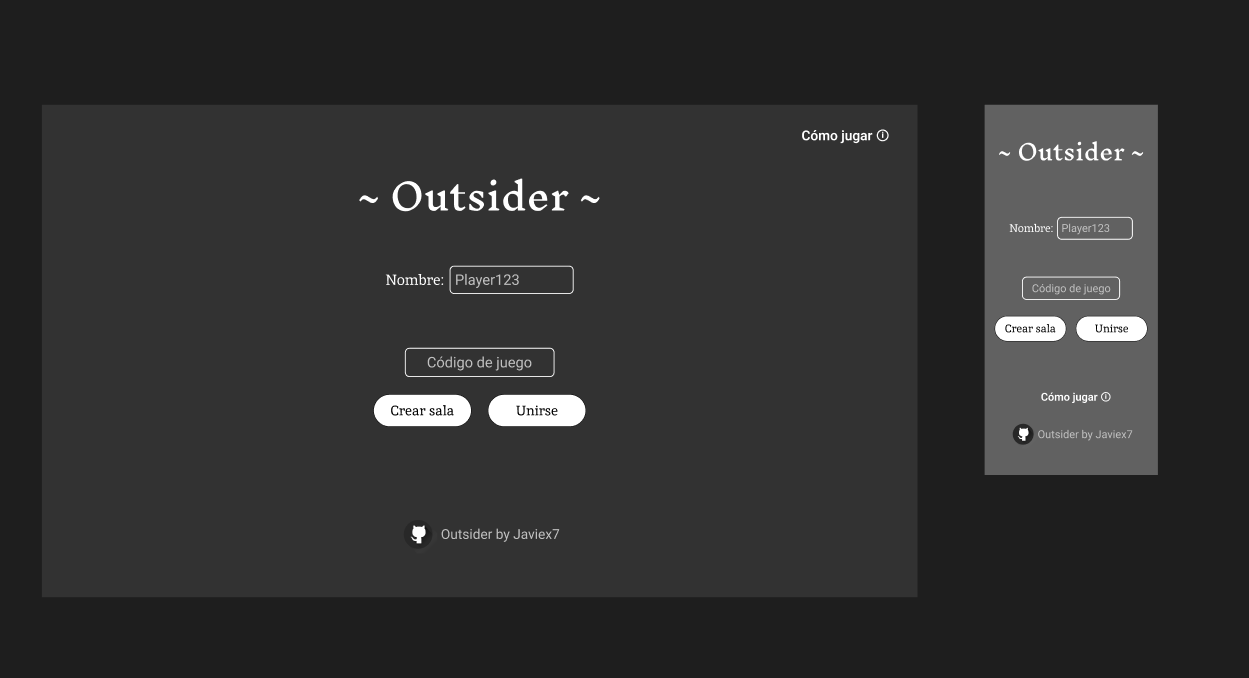
\includegraphics[height=7cm]{res_designLanding.png}
	\end{subfigure}
																																																																																																																																																																													
	\begin{subfigure}{\textwidth}
		\centering
		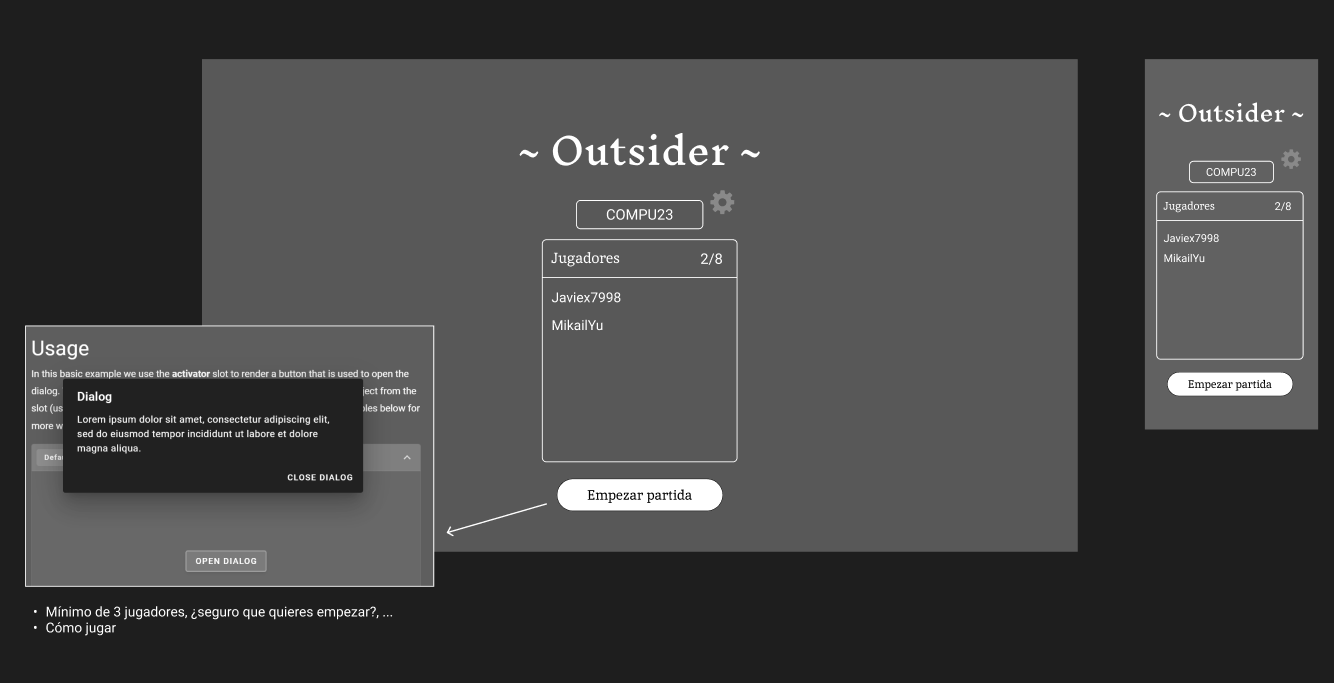
\includegraphics[height=7cm]{res_designLobby.png} 
	\end{subfigure}
																																																																																																																																																																																				
	\caption{Prototipados iniciales}
	\label{fig:res_designLanding}										
\end{figure}

Estos prototipos permiten concretar mejor el estilo y el diseño general de la página web. Además, 
se llevan a cabo varias pruebas de colores, tipografías y otros elementos estéticos antes de 
implementar estos estilos en la aplicación. En la figura \ref{fig:res_designJuego} se puede observar el primer diseño para la pantalla
de juego.

\begin{figure}[h]
	\centering
	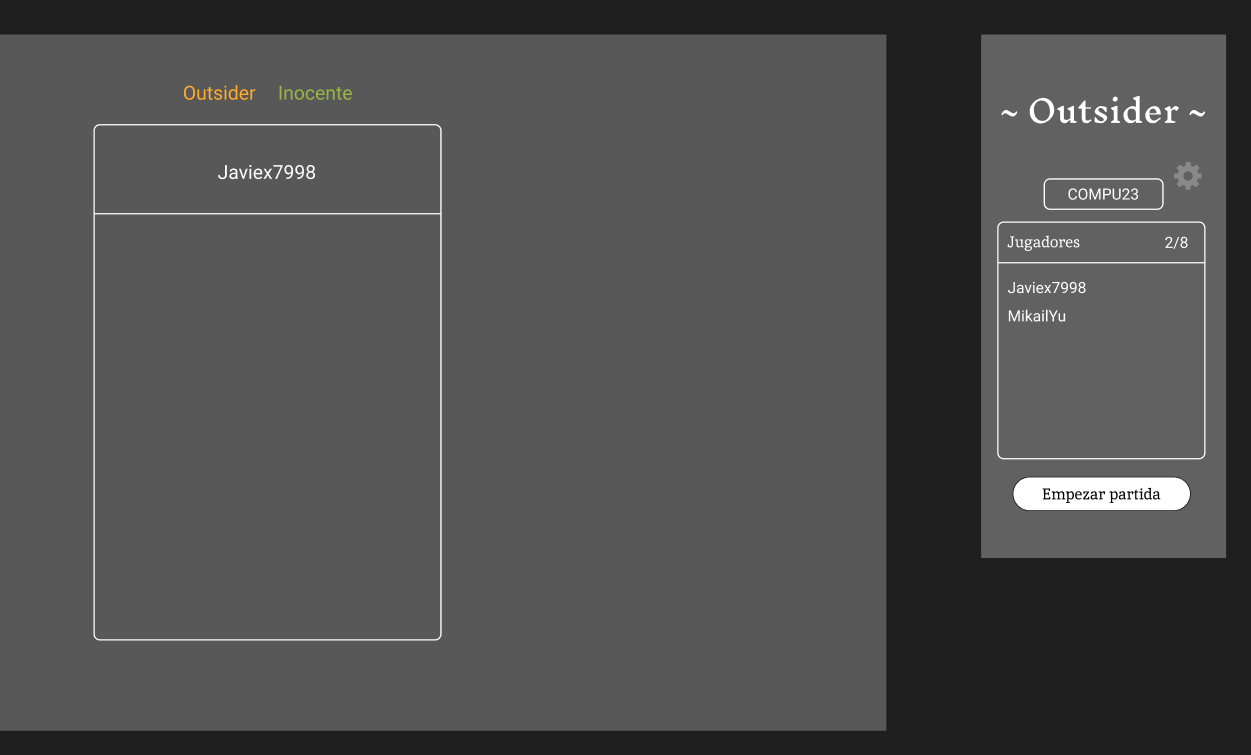
\includegraphics[height=7cm]{res_designJuego.png}
	\caption{Prototipo de la página de juego}
	\label{fig:res_designJuego}
\end{figure}

Cabría destacar que solo se ha tenido en cuenta la creación de unos pocos diseños debido a la facilidad de trabajar directamente
sobre los componentes de Vuetify y la necesidad de cambios constantes en la interfaz. De esta forma se ha evitado un 
sobreesfuerzo derivado de la iteración entre diseño e implementación.

\section{Implementación}

En esta sección se detallarán los aspectos más importantes para la implementación del sistema propuesto. 
Se abordarán tanto las funcionalidades y usos generales como los pequeños avances que se consideran significativos 
durante el proceso de desarrollo.

\subsection{Implementación básica Backend/Frontend}

La primera parte del desarrollo se ha basado en la implementación básica tanto del frontend a través de Vue como del 
backend con el uso de Django. Para esta tarea, lo más importante es la correcta instalación de depedencias así como de
la preparación del entorno de desarrollo.

Debido a la experencia previa en este apartado, no ha sido necesariamanete complicado esta instalación inicial. Para Django,
la instalación es muy sencilla, solo se necesita tener python en el sistema y ejecutar un par de mandatos, por otra parte,
la instalación de Vue puede resultar algo más complicada, y en este caso se ha optado por hacer uso directamente de Vuetify para
tener todas las dependencias derivadas de Node.js integradas en el proyecto. De esta forma se debería tener una estructura de proyecto
como la que se puede observar en la figura \ref{fig:res_designJuego}. En el directorio 'outsider' se encuentran los archivos 
de configuración base de Django, mientras que en la carpeta 'outsider-front' se encuentra todo el código fuente relacionado 
con el uso de Vue/Vuetify. 

Se destaca que Django trabaja mediante el uso de 'aplicaciones'; haciendo referencia directa a la documentación de Django: 
El término 'aplicación' o 'app' describe un paquete de Python que proporciona un conjunto de funciones en concreto. 
Estas aplicaciones suelen incluir una combinación de modelos, vistas, 
plantillas, archivos estáticos, URLs y otras configuraciones relevantes a la aplicación en concreto \cite{django}. Debido a que 
la lógica estará enfocada principalmente a la gestión de las conexiones websocket, todos los modelos de datos y en general toda 
la lógica del backend Django estará contenida dentro del directorio 'logic'.

Como se había destacado antes, dentro de la carpeta 'outsider-front', se encontrará de forma bastante desglosada todos los componentes
que conforman el frontend de Vue así como todas las configuraciones y ficheros auxiliares pertinentes. En la sección \ref{Desarrollo del frontend}
se tratará en detalle la estructura del framework de Vue/Vuetify y la construcción de la página web frontend.

De manera adicional, cabe destacar que, debido a las facilidades de mandatos que ofrecen los sistemas unix así como que el despliegue
final será en una maquina linux, se está trabajando a través de WSL, es decir,
ambas aplicaciones: frontend y backend así como sus depedencias (python y node.js principalmente) se ejecutan en ubuntu a través de la interfaz
de WSL, ya que, el ordenador en el cual se está desarrolando el proyecto solo tiene instalado Windows 11 y por decisión propia se prefiere su uso de forma
cotidiana. Es importante tener esto en cuenta en primera instancia para evitar problemas en el futuro despliegue o mientras se está trabajando en el proyecto,
debido a que, el uso de mandatos y la disponiblidad de ciertos instaladores y librerías cambia drásticamente entre Windows y Linux.

Teniendo en cuenta esta instalación y configuración básica tanto del backend como del frontend, ya se puede trabajar directamente en el desarrollo de
la aplicación per se.

\subsection{Uso y aprendizaje de tecnologías websockets} 

Después de haber configurado el entorno de desarrollo base, cabría añadir los elementos necesarios para poder 
trabajar con tecnologías asíncronas.

Para el frontend solo será necesario hacer uso de la implementación del protocolo websocket \cite{websocketMDN}, mientras que en el 
backend, como ya se había comentado, será necesario hacer uso de otros elementos, en este caso, Django Channels. 
Por ello, lo primero será realizar la instalación de Channels en el server de Django.

Además de la instalación sencilla mediante pip install, es necesaria la configuración de varios settings del proyecto, así
como implementar el uso del servidor ASGI Daphne. En la documentación \cite{djangoChannelsInstall} se indica paso a paso el proceso 
de instalación en detalle si se quiere indagar en el tema.

Con Django Channels instalado en el sistema, lo primero que se ha realizado son los propios tutoriales de uso, los cuales detallan 
la creación de un chat asíncrono, desde la configuración básica, hasta el uso de la funcionalidad de layers de forma asíncrona.

Estos tutoriales, que también se encuentran en la propia documentación de Channels \cite{djangoChannelsTutorial}, son 
de bastante calidad y se podrían comparar con la realización de una práctica guiada en una asignatura de la 
\escuelalargo. Se enseñan las capacidades básicas de los websocket y se va expandiendo a nivel funcional un ejemplo
de chat bastante completo. Se han encontrado tan interesantes estos ejemplos, que la funcionalidad backend del chat 
en la aplicación final, se ha dejado prácticamente como viene definida en estos tutoriales.

En términos generales, el funcionamiento de Channels, vendría a ser la siguiente:

\begin{itemize}
	\item En primer lugar, después de tener el proyecto configurado y una aplicación de django lista para
	      trabajar con websockets (para este proyecto será la aplicación de 'logic'), será necesario la creación de un 
	      consumidor websocket.
	\item Cuando Django acepta una solicitud HTTP, consulta la configuración de url raíz para buscar una función de vista/view y luego 
	      llama a la función de vista para manejar la solicitud. De manera similar, cuando Channels acepta una conexión WebSocket, 
	      consulta la configuración de url para buscar un consumidor y luego llama a varias funciones dentro del propio consumidor 
	      para manejar eventos de la conexión.
	\item Siendo más específicos, los consumidores se estructuran en torno a una serie de métodos/funciones con nombre correspondientes al tipo de mensaje 
	      que recibe del propio websocket. En otras palabras, se tendrá un consumidor con un método 'connect', un método 'disconnect' y un método 'receive' 
	      que gestionarán o consumirán, valga la redundancia, los mensajes de tipo websocket de nueva conexión 'new WebSocket', los de desconexión 
	      'WebSocket.close()' y los de envío de mensajes estándar 'WebSocket.send()' respectivamente.
	\item De esta forma, se entiende que los mensajes generados en el frontend web a través de la conexión websocket se 'producen' con el objetivo
	      de que el backend 'consuma' estos mensajes mediante los propios 'consumidores' que se han instanciado a la hora de crear la comunicación websocket.
	\item Como inciso final, el uso de Django Channels se basa en el uso de estos objetos consumidores de la forma que se vea 
	      más adecuada. Por ejemplo, cabe destacar que los consumidores pueden heredar de diferentes clases con diferentes características,
	      por ejemplo pueden exisitr consumidores síncronos, asíncronos, realizar decodificación JSON de forma automática, ...
\end{itemize}

Teniendo clara como funciona la lógica de consumidores, faltaría destacar la implementación propia que se ha diseñado para este proyecto: Debido a que 
la lógica gira en torno al control del flujo del juego, solo se hace uso de un controlador para gestionar la única conexión websocket que debería haber entre
un jugador y una sala de juego. Por esto útimo también se denomina al consumidor como 'RoomConsumer'. El código~\ref{alg:RoomConsumer} ejemplifica los métodos 
principales e inicialización del consumer en cuestión. Como se puede observar se ha hecho uso de un AsyncJsonWebsocketConsumer, con decodificación JSON y el uso de 
comunicación asíncrona para poder gestionar varias peticiones de forma paralela sin necesidad de esperar a que se completen las peticiones en orden.

\begin{mypython}[float={h},caption={RoomConsumer},label={alg:RoomConsumer}]
	import json
	from channels.generic.websocket import AsyncJsonWebsocketConsumer
																																																	
	from .utils.consumer_classes import State, WebsocketUser
	from .utils import sync_rest_calls, consumer_methods
	
	class RoomConsumer(AsyncJsonWebsocketConsumer):
	def __init__(self, *args, **kwargs):
																																																	
	async def connect(self): \dots																																			
	async def disconnect(self, close_code):	\dots																																			
	async def receive_json(self, content): \dots	
\end{mypython}

De esta forma el servidor es capaz de trabajar con información que le llega desde el frontend, sin embargo es necesario la capacidad opuesta, el envío de información al 
frontend desde el propio servidor, es más, debido a la lógica del juego, se debería poder enviar información a varios clientes web. Por ejemplo, a la hora de empezar una partida
a nivel lógico en el servidor, se quiere indicar a todos los jugadores que están en la sala de que ha empezado la partida así como su rol y posible contraseña.

Para empezar, se debe hacer uso del sistema de layers ya que, es indispensable para diferenciar diferentes salas de juego y permitir 
la comunicación entre diferentes instancias de consumidores, en este caso, queremos que jugadores de una misma sala se comuniquen entre sí de forma constante. 
Por ello, además de gestionar el servidor redis mediante un contenedor docker (docker run --rm -p 6379:6379 redis:7), también se tiene que procesar toda la lógica de broadcast
o envio de mensajes desde el backend al frontend. Esto se realizará mediante el propio consumidor, el cual tiene la capacidad de suscribirse a un grupo haciendo uso
de la aplicación de layers. Esta última operación se debe realizar cuando se acepta una conexión websocket en el propio consumidor. 

En el siguiente código~\ref{alg:JoinGroup} se puede observar como se hace uso del método 'channel\textunderscore layer.group\textunderscore add()' para añadir al consumidor per se 
al grupo (siempre estará relacionado el grupo a nivel lógico con la sala de juego en la que esté el propio jugador) cuando se realiza una nueva conexión websocket (método connect del consumidor). 

\begin{mypython}[float={h},caption={Añadir consumer a un grupo},label={alg:JoinGroup}]
						
	async def connect(self):
		...
		# Join room group
		await self.channel_layer.group_add(self.room_group_name, self.channel_name)
		await self.accept()
									
\end{mypython}

Por otro lado, dentro del método receive, puede ser que un usuario en concreto decida enviar el mensaje para empezar la partida y su consumidor, además de hacer la lógica de juego, 
debe hacer uso del método 'channel\textunderscore layer.group\textunderscore send()' para que los diferentes consumidores que forman parte del mismo grupo reciban la 
información de que un jugador está intentando empezar un partida. 

Este mensaje se despachará en base al 'tipo' de mensaje que defina el propio método de broadcast, es decir debe
existir un método denominado como 'startGame' el cual, además de poder realizar lógica adicional (por ejemplo, solo enviar la contraseña a jugadores Inocentes) 
enviaría finalmente el mensaje de empezar partida desde el consumidor al propio websocket (el propio usuario en el cliente web) mediante el método 'send\textunderscore json()'. 

Se puede ver de forma resumida, tanto el código de broadcast como el envío del mensaje final al cliente en el código~\ref{alg:ReceiveCode}. Para otras acciones existirán
otros métodos correspondientes y en este código solo se resalta el uso de 'startGame' para ejemplificar el uso de grupos de consumers.

Para finalizar este apartado y haciendo un poco de resumen, el objeto consumidor, además de de gestionar los mensajes que le llegan desde el cliente web y procesar la lógica necesaria, 
es capaz de enviar nueva información de vuelta a usuarios que compartan un mismo grupo, que en el contexto de este proyecto serán las salas de juego. De esta forma se logra
una comunicación bidireccional usuario-servidor con la capacidad de poder relacionar de forma consistente un grupo de conexiones en concreto.

\begin{mypython}[float={h},caption={Broadcast a todos los consumidores y envío final al cliente},label={alg:ReceiveCode}]
						
	# RECEIVE: Websocket -> Consumer -> Consumer group
	async def receive_json(self, content):
		...	
		if action == "startGame":
		self = start_game
		message = {...}
		...	
		# GROUP: Consumer -> Consumer group
		await self.channel_layer.group_send(
		self.room_group_name,
		{"type": action, "message": message, "username": username},
		)
					
	# startGame: Consumer group -> Consumer -> WebSocket
	async def startGame(self, event):
		...
		# SEND: Consumer -> WebSocket
		await self.send_json(content={...})
									
\end{mypython}

\subsection{Implementación del backend}

Habiendo explicado el funcionamiento general de Django Channels, se procede a definir en detalle los métodos y funcionalidades 
de la implementación de la lógica del juego, incluyendo elementos adicionales, como el uso de peticiones REST y teniendo en cuenta 
la legibilidad y estrucutra del código.

Para empezar, todo el código relevante que se va a tratar, pertenece a la aplicación de 'logic' dentro de la carpeta fuente del proyecto.
Dentro de esta carpeta destacamos los ficheros 'consumers.py' y 'viewsets.py'.

\begin{itemize}
	\item consumers.py - Teniendo en cuenta todo lo que se ha explicado en el apartado previo, dentro de 'consumers.py' se encuentra la lógica asociada
	 	  al consumidor websocket de la aplicación, RoomConsumer. Se destaca cada consumidor tiene una inicialización de datos que va a ir trabajando
		  a lo largo de la sesión. Estos datos debería estar sincronizados entre las diferentes instancias de consumer que pertenezcan 
		  al mismo grupo/sala, por ejemplo, la lista de jugadores Outsider o un flag booleano que indica el fin del juego. Además de estas variables el consumidor 
		  redefine con mucha lógica los métodos websocket básicos: connect, disconnect y receive (el receive se denomina json por heredar del tipo de consumidro 
		  AsyncJsonWebsocketConsumer). En el siguiente apartado se detallará la gestión de conexiones y desconexiones, pero por ahora, cabría destacar el método receive.

		  El método receive tendrá la mayor carga de lógica y es por eso que dentro de la carpeta utils (dentro de la aplicación de logic) se encontrarán
		  otros métodos auxiliares para separar mejor el código, ya que, el método receive funciona como un gran switch en base al mensaje que reciba el
		  consumidor desde websocket. Si un jugador envia el mensaje de siguiente turno (solo lo puede hacer el jugador cuyo turno este activo) el consumidor 
		  , además de gestionar la lógica pertinente para indicar que sería el turno del siguiente jugador (puede que se acabe la ronda por ejemplo), debe indicar
		  al resto de consumidores el resultado que haya sido calculado.

		  Para evitar acciones erróneas, existe una selección de acciones posibles, que serían: 'default', 'connection', 'startGame', 'nextTurn', 
		  'votingOutsider', 'lastChance', 'nextRound' y 'endGame' y estas hacen referencia a su traducción en español ('acción por defecto', 'conexión', 
		  'empezar juego', 'siguiente turno', 'votar outsider', 'última oportunidad', 'siguiente ronda' y 'final de juego'). Habiendo realizado la lógica de cada
		  acción, se le comunica al resto de consumidores la información pertinente y es por ello que se definen también todos los métodos que reciven la información
		  del grupo/sala con el mismo nombre de estas acciones. Por ejemplo, si la acción es 'votingOutsider', ese consumidor enviará un mensaje a todos los consumidores 
		  de su grupo de tipo 'votingOutsider', y cada uno de los consumidores ejecutará el método con el mismo nombre que el tipo de mensaje enviado por el consumidor original,
		  en este caso, será el método 'async def votingOutsider(self, event)'.

		  De forma extra, también se ha definido un Enum que identifica el estado de un jugador y una clase WebsocketUser que hace referencia a la información del usuario
		  que hace uso de la conexión websocket con el servidor a la hora de entrar en una sala de juego (dentro de 'utils/consumer\textunderscore classes.py'). De esta forma se 
		  facilita la lógica de la aplicación y se estructuran de forma más ordenada los datos.

	\item viewsets.py - Se está destacando muchas veces el hecho de 'entrar en una sala' por parte del usuario, pero esto no es una acción trivial, ya que, de alguna forma
		  el cliente web debería poder conocer de forma sencilla el estado de una supuesta sala si es que un usuario quiere crearla o en todo caso entrar a una. Es por ello, que se destaca la implementación
		  de una lógica basada en modelo de datos, es decir, el estado de las salas se define y actualiza en base de datos para poder gestionar de forma sencila las futuras conexiones websocket.

		  Esta lógica se realiza mediante Django estándar: Primero se definen modelos de datos, en este caso RoomModel, para guardar la información de estado de una sala/partida
		  y de forma adicional WordsListModel para definir una lista de palabras para el juego de forma persistente y fácilmente accesible. Definidos los modelos, simplemente se hace uso de ellos mediante
		  las vistas implementadas en 'viewsets.py'. Si un usuario quiere crear una sala, si no existe una sala con el mismo nombre, puede crearla sin problemas y ahora se puede gestionar sin problemas
		  la lógica websocket asociada, realizando una conexión inicial. De forma similar sin un usuario quiere entrar en una sala, se comprueba si existe para poder realizar realizar la conexión websocket.

		  Es importante destacar que se realizan peticiones a la base de datos desde el entorno asíncrono del consumidor websocket (desde 'consumers.py' 
		  y 'utils/consumer\textunderscore methods.py'), es por ello que dentro de la carpeta de utils también se define un fichero 'sync\textunderscore rest\textunderscore calls' que contiene 
		  los métodos de acceso a base de datos con un manejo específico (a través de la definición de un contexto síncrono y seguro) para que todo funcione sin problemas. Al final, es una necesidad
		  separar la lógica síncrona de la base de datos con la asíncrona de las comunicación con websockets.
	
\end{itemize}

De forma adicional destacamos la configuración básica de urls y enrutamiento, tanto para websocket (a través de 'routing.py') como para las vistas clásicas (en 'urls.py') así como de 
configuración adicional a la hora de iniciar o reiniciar el servidor backend (en 'apps.py'); esta configuración inicial se encarga de limpiar salas si se han eliminado 
de forma incorrecta debido a un bug del server o problemas de conexión mayores y, por otra parte, actualizar la lista de palabras que utiliza el juego cuando no se ha encontrado
una lista de palabras inicial válidas o se ha borrado de la base de datos en algún momento.


\subsection{Gestión de conexiones simultáneas y otros problemas generales}

En esta sección se querría destacar los principales problemas que se han ido encontrado a lo largo del desarrollo, especialmente los relacionados con 
la lógica en el backend.

\begin{itemize}
	\item En primer lugar, es muy importante tener en cuenta problemas de sincronización como salas ya creadas, o códigos no válidos. A la hora de gestionar a varios jugadores en una misma sala
		  eran recurrentes los problemas relacioandos con la información que tiene un consumidor y otro, ya que, la mayor parte de la lógica, por ejemplo, calcular el resultado de una votación
		  es una tarea que solo debería realizar un consumidor en concretro que estuviese a la espera del resto de votaciones. Por ello, se trabajó mucho en la sincronización de información
		  entre todos los consumidores, así como en la creación de una lógica de listeners robusta en el frontend; siempre a la espera de nuevos mensajes websocket provenientes del servidor.
	
		  Por otra parte, se ideó un mecanismo clave en la gestión asíncrona de la lógica del juego: Hay muchos puntos en los cuales cualquier jugador podría empezar/acabar con la partida
		  o como se acaba de comentar, hay partes de código que solo tiene sentido que gestione un usuario/consumidor en exclusiva, para no repetir cálculos y respetar una sincronía dentro
		  de la comunicación asíncrona. Este tipo de problemas pueden resultar familiares a los que hayan trabajado con este tipo de tecnologías, personalmente se pensó en soluciones como el concepto de Barrier
		  a la hora de forzar la espera de un proceso en un punto hasta que el resto de procesos hayan llegado al mismo punto \cite{Barrier}. 
		
		  Finalmente, se llegó a una solución sencila que también ayuda al diseño y experiencia de usuario: Un rol adicional de capitán o jefe de la sala. La clave radica en la sencillez de la idea, 
		  el primer jugador que entra en una sala (el creador) es el capitán de la sala, y eso le permite iniciar la partida y tener la capacidad de terminarla entre rondas. De esta forma, gran parte de lógica la asume el 
		  consumidor del websocket asociado al usuario capitán. El único problema es la posible desconexión de este capitán, por ello, una gran parte del desarrollo ha sido la correcta sincronización de conexiones dentro 
		  de la sala. Para evitar posibles problemas en la lógica del juego, si un jugador (que no ha sido eliminado y no está como espectador en el juego) se desconecta en mitad de partida, se cancela la partida 
		  y los jugadores vuelven a la página principal.
		
		  Esto es debido a que recalcular la lógica en mitad de partida se hace demasiado complicada, especialmente mostrar los cambios de forma visual y sencilla a los usuarios. Por otra parte, las partidas son
		  absurdamente rápidas y sencillas y se persigue un trato de la información sencillo y poco persistente. Solo exisite información de los usuarios mientras están en una sala de juego, si se cierra la página 
		  web no hay ninguna traza de información que se haya almacenado obviando el historial de navegación y los datos asociados a la caché del propio navegador.

	\item Dicho esto, se querría hablar también sobre la gestión de resultados de las rondas, ya que, también ha sido un apartado un poco tedioso. El juego funciona de forma sencila, pero con todas las reglas aplicadas
		  hay diversos resultados a la hora de tratar la información de votación de los jugadores, desde empates, hasta la imposibilidad de seguir jugando de forma coherente (mismo número de outsiders que de jugadores).
		  Por ende, es importante tener en cuenta lo complicado que se puede volver un simple diálogo de texto y tener en cuenta todos los resultados posibles. En este aspecto el testing automático puede facilitar las
		  cosas y por ello puede resultar bastante úitl aplicarlo desde un primer momento.

	\item Finalmente también se desearía discutir sobre un elemento menor: La lista de palabras. El juego debería proporcionar una lista de palabras para que los usuarios jueguen con las 
		  diversas contraseñas, de forma adicional, se ha querido poder modificar esa lista de palabras de forma sencilla mediante el administrador de Django y un campo JSON (en el apéndice se indicará en mayor detalle su uso).
		  Dicho esto, se ha ido modificando una regla que indica que se le debe proporcionar al jugador Outsider una 'contraseña falsa' si es el primer jugador en una ronda; esto es porque si 
		  no tiene ninguna clase de pista adicional, se hace complicado evitar ser descubierto como Outsider. Por ende, la lista de palabras se hace algo más compleja, ya que, en este caso, el Outsider
		  debería tener otra palabra que se parezca a nivel semántico a la contraseña, pero sin ser la propia contraseña; por ello, para generar esta lista de tuplas se ha hecho uso de ChatGPT \cite{ChatGPT} para
		  poder tener al menos unos datos iniciales con los que testear y mostrar la aplicación evitando palabras repetidas entre diferentes partidas. Igualmente esto sería un aspecto a mejorar e incluso
		  se podrían modificar las reglas para poder tratar con este aspecto en especial., porque, incluso haciendo uso de IA, se ha hecho muy poco consistente esta generación de tuplas de palabras semánticamente similares.
		
\end{itemize}


\subsection{Desarrollo del frontend} \label{Desarrollo del frontend}

Una vez explicado el desarrollo relacionado con el servidor/backend, se puede comenzar a abordar el desarrollo del frontend utilizando Vue
y las tecnologías web pertinentes. Para comenzar, todo el código del que se va a hablar se encuentro dentro de la carpeta 'outsider-front' dentro de la carpeta
principal del proyecto. Dentro de este directorio están los archivos específicos del proyecto (principalmente en la carpeta src), junto con las librerías de Node.js y otras 
configuraciones adicionales.

Vue solo hace una gran distinción entre elementos: páginas y componentes, que se distinguen por su uso específico. La diferencia es simplemente que 
las vistas son componentes con capacidad de enrutamiento; es decir, mientras que los componentes pueden actuar como bloques reutilizables de comportamiento, estilo 
y estructura en diversas partes de la página web, las vistas tienen una ruta específica dentro de la página web. En el desarrollo del proyecto, como se pude observar 
en la siguiente figura (\ref{fig:res_estructFronted}), se han planteado dos vistas que definen la pagían de inicio y la página que gestiona la sala de juego. Por otra parte
existen diversos componentes reutilizables que se integran dentro de cada una de la vistas.

\begin{figure}[h]
	\centering
	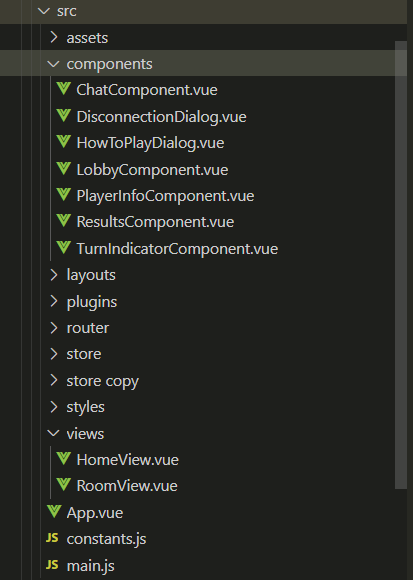
\includegraphics[height=10cm,clip=true]{res_estructFronted.png}
	\caption{Estructura de ficheros en el frontend}
	\label{fig:res_estructFronted}
\end{figure}

Antes de continuar con la descripción de las vistas, cabría destacar nuevamente el uso de Vuetify, ya que, se ha utlizado en gran medida para facilitar 
el trabajo de diseño y maquetación web. Esto se ha llevado a cabo principalmente mediante el uso de componentes de Vuetify; estos componentes de diferentes tipos, facilitan la
construcción de interfaz facilitando elementos como botones, carrouseles de elementos, menús, ... con la facilidad de cambiar su diseño de forma sencilla sin hacer uso
extensivo de CSS o en todo caso de código adicional para definir animaciones y comportamientos. De esta forma, se consigue una interfaz visualmente atractiva y de sencilla
creación.

Dicho esto, en la figura (\ref{fig:res_mainpage}) se puede observar la vista principal, 'HomeView.vue' en un dispositivo de escritorio. Es una vista muy sencilla y el código asociado no
es nada complejo, ya que solo tiene en cuenta la actuación de los botones para crear una sala y unirse a una sala mediante una petición sencilla al servidor con el uso de axios \cite{vueAxios}. 
Se tiene en cuenta que el nombre de usuario no sea ni demasiado corto, ni demasiado largo así como que el código de sala esté presente a la hora de intentar acceder a una sala de juego 
(o intentar crearla). También se proporcionan mensajes de 'error' si ha habido alguna incidencia (normalmente el intertar unirse a una sala que no existe o al intentar crear una sala ya existente). 
Para finalizar, la página también muestra con mucho detalle un diálogo con todas las instrucciones del juego si se pulsa el botón de 'Cómo jugar'.

\begin{figure}[h]
	\centering
	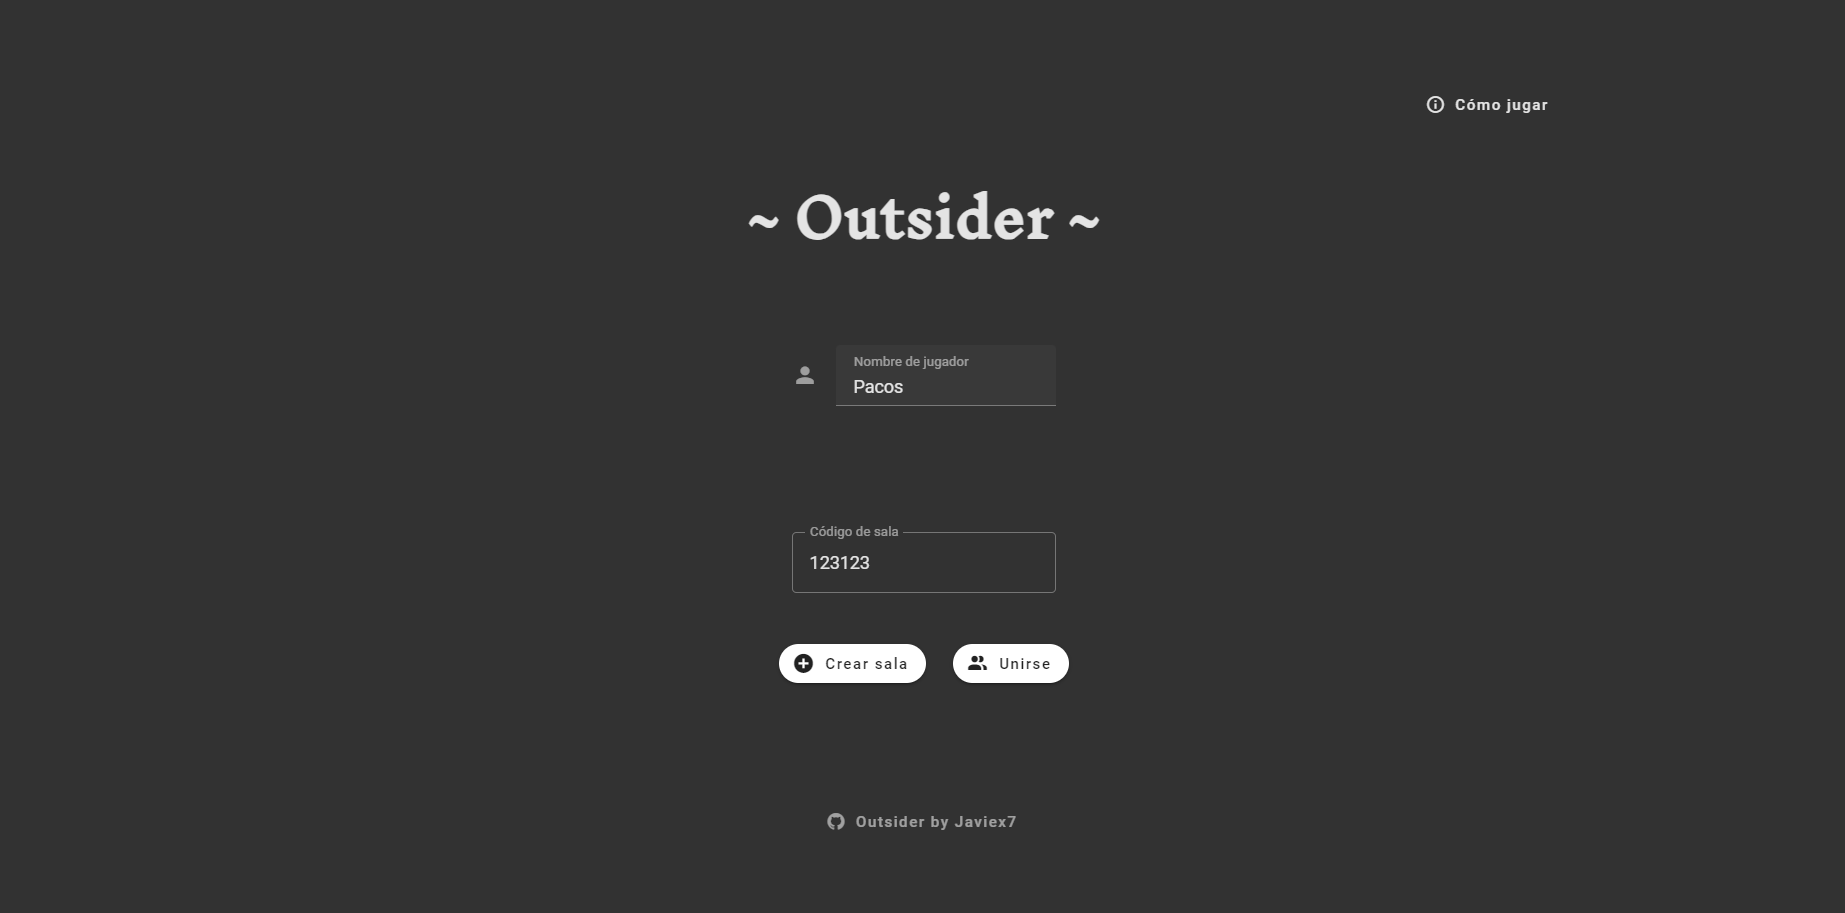
\includegraphics[width=\textwidth,clip=true]{res_mainpage.png}
	\caption{Página principal}
	\label{fig:res_mainpage}
\end{figure}

La otra vista, 'RoomView.vue', bastante más compleja, maneja toda la interfaz gráfica así como la lógica de peticiones websocket asociadas al juego per se, desde la
visualización y funcionamiento del chat, hasta la correcta presentación de los resultados de una ronda.

Para empezar, destacamos el LobbyComponent, encargado de mostrar y gestionar, dentro de la vista de la sala todos los elementos relacionados con la sala de espera, etre los que se
incluye un chat entre los miembros actuales de la sala, diferentes indicadores del estado de la sala (código de sala para que se puedan unir otros usuarios, número de jugadores y
lista con indicadores sobre capitanía de la sala) y un botón que sirve para iniciar la partida por parte del capitán de la sala si hay más de dos usuarios presentes.

En la figura (\ref{fig:res_lobby}) se puede ver un lobby/sala de dos jugadores interactuando con el chat así como otra sala con seis jugadores listos para jugar. De esta sección solo
cabría resaltar que se indica cuando se jugará con un outsider adicional (con seis o más jugadores) y también que, al lado de cada nombre de usuario se indica quién es el capitán mediante
un logo de corona y resaltado en azul además de quién es el propio usuario que está haciendo uso de la aplicación mediante otro icono de cuenta/usuario al lado del nombre introducido
antes de ingresar en la sala.

\begin{figure}[h]
   \centering
   \begin{minipage}{0.45\textwidth}
	\centering
	  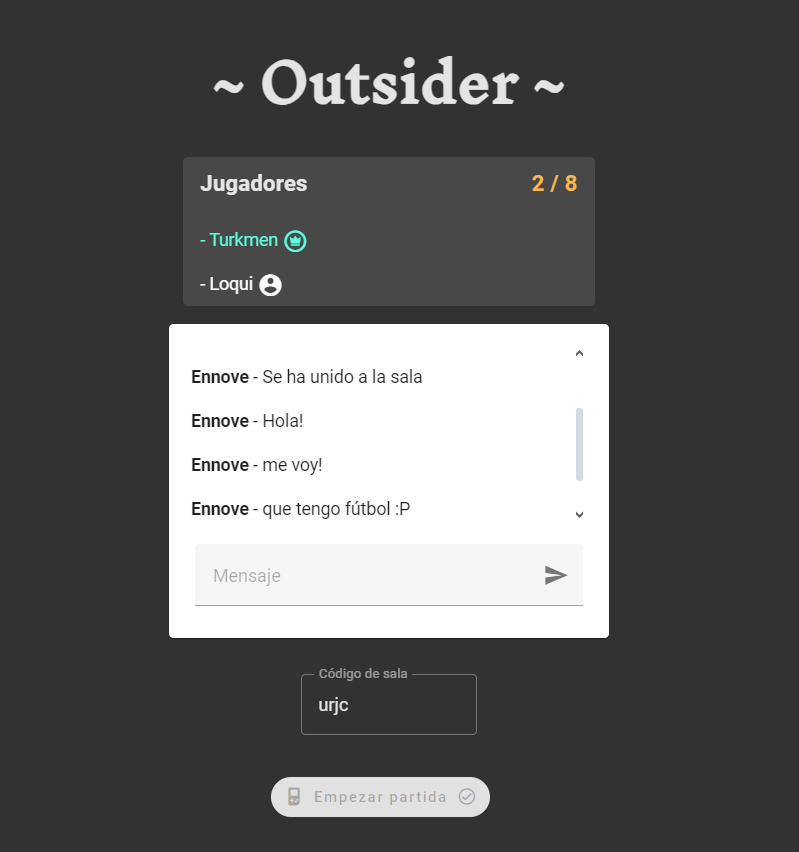
\includegraphics[clip=true,width=\textwidth]{res_lobby2.png}\\
   \end{minipage}
   \hfill
   \begin{minipage}{0.45\textwidth}
	\centering
	  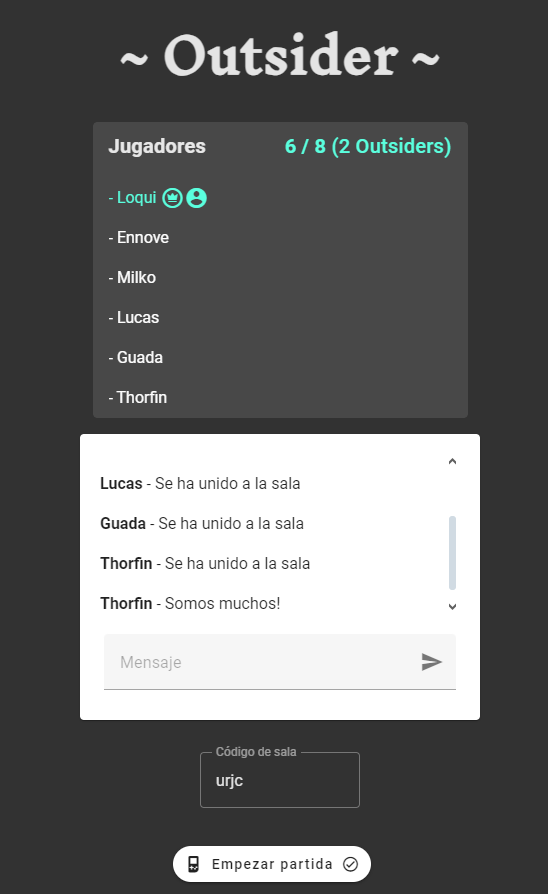
\includegraphics[clip=true,width=\textwidth]{res_lobby1.png}\\
   \end{minipage}
   \caption{Sala de espera con diferentes números de usuarios}
   \label{fig:res_lobby}
 \end{figure}

\section{Testing}

\section{Pruebas con usuarios}

\section{Despliegue}







% Capítulo 5
\chapter{Conclusiones y trabajos futuros}
\label{chap:conclusiones}
En este capítulo se detallan las conclusiones derivadas del TFG y la propuesta de posibles trabajos futuros.

\section{Texto de relleno}

\lipsum[1-18]

\blankpage

%%%%%%%%%%%%%%%%%%%%%%%%%%%%%%% Bibliografía %%%%%%%%%%%%%%%%%%%%%%%%%%%%%%%

\phantomsection
\addcontentsline{toc}{chapter}{Bibliografía}

\footnotesize{
	%\bibliographystyle{hispa}
	\bibliographystyle{IEEEtran}
	\bibliography{bibliografia}
}

% No expandir elementos para llenar toda la página
\raggedbottom
\afterpage{\blankpage}

\newpage


%%%%%%%%%%%%%%%%%%%%%%%%%%%%%%% Apéndices %%%%%%%%%%%%%%%%%%%%%%%%%%%%%%%

\appendix

\phantomsection
\addcontentsline{toc}{chapter}{Apéndices}

\mbox{}
\vfill
\begin{center}
	\begin{Huge}
		\textbf{Apéndices}
	\end{Huge}
\end{center}
\vfill
\mbox{}
\thispagestyle{empty}

\newpage
\mbox{}
\thispagestyle{empty}
\newpage

\chapter{Esquemas y recursos adicionales}
\section{Ejemplo de sección}

Sección del apéndice\tutor{Aquí deberías contar, por ejemplo, como lanzar tu aplicación en local y en AWS (pueden ser varios anexos)}


\chapter{Instrucciones de testing y despliegue de la aplicación}
\section{Tutorial de testing}
\label{sect:testing}

En este apartado se indican los pasos a seguir para poder ejecutar los tests de la aplicación sin complicaciones. Se recomienda hacer
la configuración necesaria en un sistema Unix ya que es donde se ha trabajado la aplicación y, más adelante, se indicará hacer uso de mandatos 
específicos de Unix.

\begin{enumerate}
	\item Lo primero es tener el proyecto actualizado. El repositorio debería ser accesible para cualquier usuario en 
            \href{https://github.com/Javiex7/Outsider}{github.com/Javiex7/Outsider}.
	\item Para la ejecución de los tests en indispensable la instalación tanto de Python \cite{installPython} como de Docker \cite{installDocker}.
	\item Con estos programas instalados en el sistema, es necesario acceder al repositorio para la configuración básica.
	\item Dentro del proyecto, son necesarios la instalación de varios elementos en el dispositivo, específicamente Django y los paquetes
	      pertinentes. Para evitar problemas, se recomienda descargar los elementos listados en el ``requirements.txt'' dentro de la carpeta principal
	      ``OutsiderProject''. Esta instalación se puede realizar fácilmente mediante el mandato: 
	      	                
	      pip install -r requirements.txt
	      	      
	\item A continuación, se requiere ejecutar un contenedor en Docker encargado de gestionar el servidor Redis para
	      que se haga uso en los tests. Mediante el siguiente mandato se puede poner en ejecución el servicio:
	      	      
	      docker run --rm -p 6379:6379 redis:7
	      	      
	\item Antes de poder ejecutar los tests, se debe configurar un variable de entorno para indicar el uso de 
	      este servidor Redis. Para ello habría que acceder a ``OutsiderProject/outsider/settings.py'' y modificar
	      el flag booleano denominado ``TEST'' y asegurarse que su valor sea True (línea 92).
	      	      
	\item Finalmente, el sistema puede ejecutar los tests. Para ello solo habría que ejecutar el mandato ``pytest''
	      desde el directorio padre, ``OutsiderProject''. Después de la ejecución debería mostrarse por consola
	      un resultado similar a lo que se puede visualizar en la Figura \ref{fig:res_testing}
	      	         
\end{enumerate}	

\begin{figure}[h]
	\centering
	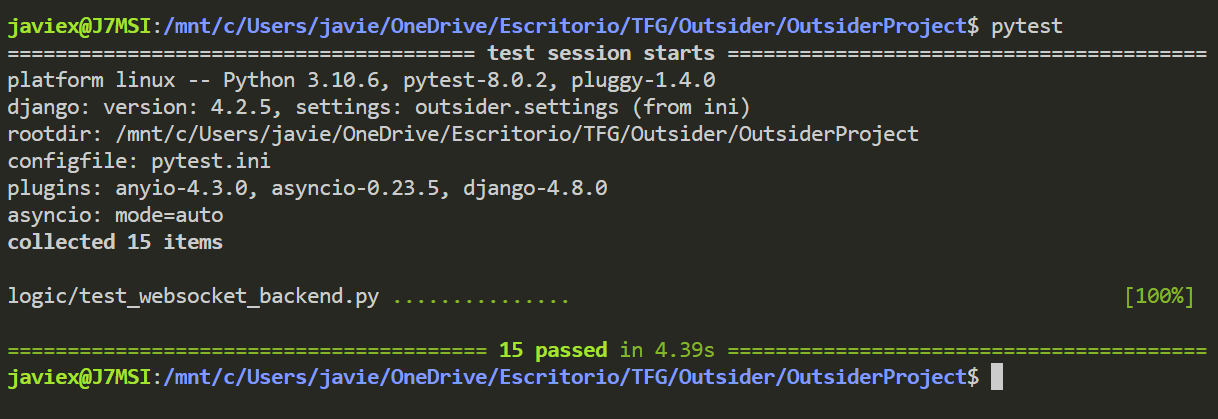
\includegraphics[width=\textwidth,clip=true]{res_testing.png}
	\caption{Ejecución de tests}
	\label{fig:res_testing}
\end{figure}


% Fin del documento
\end{document}
